\documentclass[11pt]{amsart}
%\linespread{1.25}
\usepackage[margin=3.5cm]{geometry}

\usepackage[noend,boxruled]{algorithm2e}
%Customize appearance using line below:
\SetKwFor{For}{\normalfont{for}}{:}{endfor}

\usepackage[english]{babel}
\usepackage{appendix}
\usepackage{amsmath}
\usepackage{amsfonts}
\usepackage{amssymb}
%\usepackage{showlabels}
\usepackage{amsthm}
\usepackage{marginnote}
\usepackage{stmaryrd}
\usepackage{enumitem}
\usepackage[english]{babel}
\usepackage{yfonts}
\usepackage[T1]{fontenc}
\usepackage[utf8x]{inputenc}
\usepackage[normalem]{ulem}

\renewcommand\thepart{\Roman{part}}

%This reverse-links the references in the paper. Useful for large papers.
\usepackage[backref]{hyperref}
\hypersetup{
  colorlinks   = true,          %Colors links instead of ugly boxes
  urlcolor     = violet,          %Color for external hyperlinks
  linkcolor    = violet,          %Color of internal links
  citecolor   = blue             %Color of citations
}

\usepackage{calrsfs}
\DeclareMathAlphabet{\pazocal}{OMS}{zplm}{m}{n}

\usepackage{verbatim}
\usepackage{graphicx}
\usepackage{verbatim}
\usepackage{faktor}
\usepackage{xcolor}
\usepackage{xfrac}
\usepackage{tikz,tikz-cd}
\usetikzlibrary{decorations.pathmorphing,decorations.pathreplacing,patterns,arrows.meta}


\definecolor{red}{rgb}{1,0,0}

\usepackage[all]{xy}
\usepackage{bbm}
\usepackage{tabularx}
\usepackage{longtable}
\usepackage{tabu}
\usepackage{booktabs}
\usepackage{mathtools}

\usepackage[]{textcomp}
\usepackage[sups]{Baskervaldx}
\usepackage{cabin}
\usepackage[varqu,varl]{inconsolata}
\usepackage[baskervaldx,bigdelims,vvarbb]{newtxmath}
\usepackage[cal=cm]{mathalfa}


\newcommand{\plC}{\scalebox{0.8}[1.3]{$\sqsubset$}}
\newcommand{\sidenote}[1]{\marginpar{\textbf{\color{red}#1}}}
\newcommand{\lcm}{\operatorname{lcm}}

% FIGURES FOR USE LATER
%%%%%%%%%%%%%%%%%%%%%%%%%%%%%%%%%%%%%%%%%%%%%%%%%%%%%%%%%%%%
\def\Yagraph{\tikz[baseline=-3pt,scale=.8]{
\draw (2,0) -- (0,1) (2,0) -- (0,.5) (2,0) -- (0,-1);
\draw (2,0) circle(2pt)[fill=black];
\draw [->] (2,0) -- (2.7,0);
\draw (2.6,0) node[right]{\tiny{$x_k$}};
\draw (0,1) circle(2pt)[fill=white];
\draw (0,.5) circle(2pt)[fill=black];
\draw (0,-.25) node{$\vdots$};
\draw (0,-1) circle(2pt)[fill=black];
\draw [blue,fill=blue] (0,-2) circle[radius=2pt];
\draw [->,blue,thick] (0,-2) -- (3,-2);
\draw [blue,fill=blue] (2,-2) circle[radius=2pt];
\draw [->,blue] (1,-0.9) -- (1,-1.6);

\draw [blue] (2,-2) node[above]{\tiny$\diamond$};
\draw [blue] (0,-2) node[above]{\tiny$0$};

\draw (2.05,0) node[above]{\tiny{$\sqC_0$}};
\draw (0,1) node[left]{\tiny{$\sqC_1$}};
\draw (0,.5) node[left]{\tiny{$\sqC_2$}};
\draw (0,-1) node[left]{\tiny{$\sqC_r$}};
}}

\def\Ybgraph{\tikz[baseline=-3pt,scale=.8]{
\draw (2,0) to[out=120,in=0] (0,1) (2,0) -- (0,1) (2,0) -- (0,.5) (2,0) -- (0,-1);
\draw (2,0) circle(2pt)[fill=black];
\draw [->] (2,0) -- (2.7,0);
\draw (2.6,0) node[right]{\tiny{$x_k$}};
\draw (0,1) circle(2pt)[fill=black];
\draw (0,.5) circle(2pt)[fill=black];
\draw (0,-.25) node{$\vdots$};
\draw (0,-1) circle(2pt)[fill=black];
\draw [blue,fill=blue] (0,-2) circle[radius=2pt];
\draw [->,blue,thick] (0,-2) -- (3,-2);
\draw [blue,fill=blue] (2,-2) circle[radius=2pt];
\draw [->,blue] (1,-0.9) -- (1,-1.6);
\draw [blue] (2,-2) node[above]{\tiny$\diamond$};
\draw [blue] (0,-2) node[above]{\tiny$0$};

\draw (2.05,0) node[above]{\tiny{$\sqC_0$}};
\draw (0,1) node[left]{\tiny{$\sqC_1$}};
\draw (0,.5) node[left]{\tiny{$\sqC_3$}};
\draw (0,-1) node[left]{\tiny{$\sqC_r$}};
}}

\def\Ycgraph{\tikz[baseline=-3pt,scale=.8]{
\draw (2,0) -- (0,1) (2,0) -- (0,.5) (2,0) -- (0,-1);
\draw [->] (2,0) -- (2.7,0);
\draw (2.6,0) node[right]{\tiny{$x_k$}};
\draw (2,0) circle(2pt)[fill=white];
\draw (0,1) circle(2pt)[fill=black];
\draw (0,.5) circle(2pt)[fill=black];
\draw (0,-.25) node{$\vdots$};
\draw (0,-1) circle(2pt)[fill=black];
\draw [blue,fill=blue] (0,-2) circle[radius=2pt];
\draw [->,blue,thick] (0,-2) -- (3,-2);
\draw [blue,fill=blue] (2,-2) circle[radius=2pt];
\draw [blue] (2,-2) node[above]{\tiny$\diamond$};
\draw [blue] (0,-2) node[above]{\tiny$0$};
\draw [->,blue] (1,-0.9) -- (1,-1.6);

\draw (2.05,0) node[above]{\tiny{$\sqC_0$}};
\draw (0,1) node[left]{\tiny{$\sqC_1$}};
\draw (0,.5) node[left]{\tiny{$\sqC_2$}};
\draw (0,-1) node[left]{\tiny{$\sqC_r$}};
}}
%%%%%%%%%%%%%%%%%%%%%%%%%%%%%%%%%%%%%%%%%%%%%%%%%%%%%%%%%%%%%%

\newcommand{\tred}{\textcolor{red}}
\newcommand{\mathsq}[1]{#1}

\newcommand{\sqC}{\scalebox{0.8}[1.3]{$\sqsubset$}}
\newcommand{\Kim}{\operatorname{Kim}}
\newcommand{\ACGS}{\operatorname{ACGS}}

\newcommand{\pM}{\pazocal{M}}
\newcommand{\TT}{\operatorname{T}}
\newcommand{\oM}{\overline{\mathcal{M}}}
\newcommand{\M}[4]{\overline{\mathcal{M}}_{#1,#2}(#3,#4)}

\newcommand{\Mlog}[4]{\overline{\mathcal{M}}^{\operatorname{log}}_{#1,#2}(#3,#4)}
\newcommand{\MLog}{\overline{\mathcal{M}}^{\operatorname{log}}}
\newcommand{\Mpunct}[4]{\overline{\mathcal{M}}^{\operatorname{punct}}_{#1,#2}(#3,#4)}
\newcommand{\MG}[4]{\overline{\mathcal{M}}^{\rm G}_{#1,#2}(#3,#4)}
\newcommand{\Q}[4]{\mathcal{Q}_{#1,#2}(#3,#4)}
\newcommand{\Qe}[4]{\mathcal{Q}^{\epsilon}_{#1,#2}(#3,#4)}
\newcommand{\Qt}[4]{\widetilde{\mathcal Q}_{#1,#2}(#3,#4)}
\newcommand{\QG}[4]{\mathcal{Q}G_{#1,#2}(#3,#4)}
\newcommand{\QGe}[4]{\mathcal{Q}G^{\epsilon}_{#1,#2}(#3,#4)}
\newcommand{\D}[3]{\mathcal{D^Q}(#1,#2,#3)}
\newcommand{\E}[3]{\mathcal{E^Q}(#1,#2,#3)}
\newcommand{\PP}{\mathbb P}
\newcommand{\Z}{\mathbb{Z}}
\newcommand{\VZ}{\pazocal{V\!Z}}
\newcommand{\tVZc}[4]{\widetilde{\mathcal{V\!Z}}^{\rm{ctr}}_{#1,#2}(#3,#4)}
\newcommand{\VZc}[4]{\mathcal{V\!Z}_{#1,#2}(#3,#4)}
\newcommand{\VZcLi}[4]{\mathcal{V\!Z}^{\rm{ctr, Li}}_{#1,#2}(#3,#4)}
\newcommand{\VZrel}[4]{\mathcal{V\!Z}^{\rm{rel}}_{#1,#2}(#3,#4)}
\newcommand{\stab}{\rm{stab}}
\newcommand{\st}{\star}
\newcommand{\stC}{C'}
\newcommand{\stpi}{\pi'}
\newcommand{\sts}{s'}
\newcommand{\N}{\mathbb{N}}
\newcommand{\OO}{\mathcal{O}}
\renewcommand{\to}{\rightarrow}
\newcommand{\A}{\mathcal A}
\newcommand{\B}{\mathcal B}
\newcommand{\C}{\mathfrak C}
\newcommand{\cC}{\mathcal C}
\newcommand{\EE}{\mathbf{E}}
\renewcommand{\L}{\mathcal L}
\newcommand{\LL}{\mathbf{L}}
\newcommand{\MM}{\mathfrak M}
\newcommand{\Aaff}{\mathbb{A}}
\newcommand{\kfield}{\Bbbk}
\newcommand{\comp}{\chi}
\newcommand{\sst}{\sigma^{\operatorname{ss}}}
\newcommand{\Pic}{\operatorname{Pic}}
\newcommand{\Def}{\operatorname{Def}}
\newcommand{\Spec}{\operatorname{Spec}}
\newcommand{\Proj}{\operatorname{Proj}}
\newcommand{\Hom}{\operatorname{Hom}}
\newcommand{\Ext}{\operatorname{Ext}}
\newcommand{\Gm}{\mathbb{G}_{\text{m}}}
\newcommand{\virt}[1]{[#1]^{\operatorname{virt}}}
\newcommand{\vip}[1]{[#1]^{\operatorname{prod}}}
\newcommand{\Id}{\operatorname{Id}}
\newcommand{\CC}{\mathbb{C}}
\newcommand{\QQ}{\mathbb{Q}}
\newcommand{\HH}{\operatorname{H}}
\newcommand{\Glog}{\mathbb{G}_{\mathrm{log}}}
\newcommand{\Achow}{\operatorname{A}}
\newcommand{\pt}{\operatorname{pt}}
\newcommand{\bq}{\begin{equation}}
\newcommand{\eq}{\end{equation}}
\newcommand{\ba}{\begin{aligned}}
\newcommand{\ea}{\end{aligned}}
\newcommand{\be}{\begin{enumerate}}
\newcommand{\ee}{\end{enumerate}}
\newcommand{\bsm}{\left(\begin{smallmatrix}}
\newcommand{\esm}{\end{smallmatrix}\right)}                   
\newcommand{\bpm}{\begin{pmatrix}}
\newcommand{\epm}{\end{pmatrix}}
\newcommand{\barr}{\begin{displaymath}\begin{array}{cccc}}
\newcommand{\earr}{\end{array}\end{displaymath}}
\newcommand{\barrl}{\begin{displaymath}\begin{array}{lcl}}
\newcommand{\earrl}{\end{array}\end{displaymath}}
\newcommand{\barl}{\begin{displaymath}\begin{array}{l}}
\newcommand{\earl}{\end{array}\end{displaymath}}
\newcommand{\bxym}{ \begin{displaymath}\xymatrix }
\newcommand{\exym}{\end{displaymath}}
\newcommand{\bcd}{\begin{center}\begin{tikzcd}}
\newcommand{\ecd}{\end{tikzcd}\end{center}}
\newcommand{\R}{\operatorname{R}^{\bullet}}
\newcommand{\dvr}{\Delta}
%\newcommand{\sslash}{\mathbin{/\mkern-6mu/}}
\newcommand{\tr}{{\rm tr}}
\newcommand{\Isom}{\text{Isom}}
\newcommand{\pr}{\operatorname{pr}}
\newcommand{\ev}{\operatorname{ev}}
\newcommand{\fgt}{\operatorname{fgt}}
\newcommand{\codim}{\operatorname{codim}}
\newcommand{\vdim}{\operatorname{vdim}}
\newcommand{\ildef}[1]{\emph{#1}}
\newcommand{\om}[1]{\mathcal{#1}}
\newcommand{\h}{\operatorname{h}}
\newcommand{\Aut}{\operatorname{Aut}}
\newcommand{\Acal}{\mathcal{A}}
\newcommand{\Scal}{\mathcal{S}}
\newcommand{\Mcal}{\mathcal{M}}
\newcommand{\Dcal}{\mathcal{D}}
\newcommand{\Ecal}{\mathcal{E}}
\newcommand{\Ncal}{\mathcal{N}}
\newcommand{\Fcal}{\mathcal{F}}
\newcommand{\Lcal}{\mathcal{L}}
\newcommand{\Ccal}{\mathcal{C}}
\newcommand{\Pcal}{\mathcal{P}}
\newcommand{\Ycal}{\mathcal{Y}}
\newcommand{\cchern}{\mathrm{c}}
\newcommand{\ol}[1]{\overline{#1}}
\newcommand{\ul}[1]{\underline{#1}}
\newcommand{\op}[1]{\operatorname{#1}}
\newcommand{\gp}{\operatorname{gp}}
\newcommand{\RR}{\mathbb{R}}
\newcommand{\NN}{\mathbb{N}}
\newcommand{\ovm}[1]{\overline{\mathcal{#1}}}
\newcommand{\ovt}[1]{\widetilde{\mathcal{#1}}}
\newcommand{\ov}[1]{\overline{#1}}

\theoremstyle{definition}
\newtheorem{thm}{Theorem}[section]
\newtheorem{lem}[thm]{Lemma}
\newtheorem{lemma}[thm]{Lemma}
\newtheorem{prop}[thm]{Proposition}
\newtheorem{cor}[thm]{Corollary}
\newtheorem*{teo*}{Theorem}
\newtheorem{ipotesi}{ipotesi}
\newtheorem*{nota}{Nota}
\newtheorem{claim}{Claim}
\newtheorem{question}[thm]{Question}
\newtheorem{conj}[thm]{Conjecture}
\newtheorem{notation}[thm]{Notation}

\newtheorem{innercustomthm}{Theorem}
\newenvironment{customthm}[1]
  {\renewcommand\theinnercustomthm{#1}\innercustomthm}
  {\endinnercustomthm}

\theoremstyle{definition}
\newtheorem{example}[thm]{Example}
\newtheorem{ex}[thm]{Example}
\newtheorem{dfn}[thm]{Definition}
\newtheorem{definition}[thm]{Definition}
\newtheorem{aside}[thm]{Aside}
\newtheorem{remark}[thm]{Remark}
\newtheorem{com}[thm]{Comment}
\newtheorem{num}{Number}
\newtheorem*{sketch}{Sketch}
\newtheorem*{rem}{Remark}
\newtheorem*{aside*}{Aside}
\newtheorem*{acknowledgements}{Acknowledgements}

\newlist{steps}{enumerate}{1}
\setlist[steps, 1]{label = Step (\arabic*):}

\newcommand{\ilemph}[1]{\emph{#1}}

\setcounter{tocdepth}{1}

\newcommand{\todo}[1]{\vspace{5mm}\par \noindent
\framebox{\begin{minipage}[c]{0.95 \textwidth} \tt #1\end{minipage}} \vspace{5mm} \par}

\def\ti{-\allowhyphens}
\newcommand{\thismonth}{\ifcase\month % case 0 --- impossible!
  \or January\or February\or March\or April\or May\or June%
  \or July\or August\or September\or October\or November%
  \or December\fi}
\newcommand{\thismonthyear}{{\thismonth} {\number\year}}
\newcommand{\thisdaymonthyear}{{\number\day} {\thismonth} {\number\year}}

\title[Curve counting in genus one: elliptic singularities and relative geometry]{Curve counting in genus one: elliptic singularities {\it \&} relative geometry}
\author{Luca Battistella, Navid Nabijou and Dhruv Ranganathan}
\date{\thismonthyear}

\begin{document}


\begin{abstract}
We construct and study the reduced, relative, genus one Gromov--Witten theory of very ample pairs. These invariants form the principal part contribution to relative Gromov--Witten theory in genus one and are relative versions of Zinger's reduced Gromov--Witten invariants. The relative and absolute theories are related by degeneration of the tangency conditions, and the resulting formulas generalize a well-known recursive calculation scheme put forward by Gathmann in genus $0$. {The geometric input is a desingularization of the principal component of the moduli space of genus one logarithmic stable maps to a very ample pair, using the geometry of elliptic singularities. Our study passes through general techniques for calculating integrals on logarithmic blowups of moduli spaces of stable maps, which may be of independent interest.}
\end{abstract}

\maketitle

\appendixtitletocoff
\tableofcontents

\setcounter{section}{-1}
\section{Introduction}

The Kontsevich moduli space of stable maps from genus $0$ curves to projective space exhibits remarkable geometry -- it is a smooth orbifold with a ``self-similar'' normal crossings boundary. These facts have combined to produce a very {satisfactory} understanding of Gromov--Witten theory in genus $0$. 

While the higher genus situation is much more difficult, in the last several years, substantial theory has been developed towards a conceptual understanding of the genus one case. This began over a decade ago with the pioneering work of Li, Vakil, and Zinger~\cite{redgone,VZ,LZ,lz2,zingerstvsred,zingred}, and was recently reinvigorated involving ideas from logarithmic geometry and singularity theory~\cite{BCM18,CM18,HL,RSPW,RSPW2,SMY1,VISC}. The result is a \textit{reduced} Gromov--Witten theory, which removes certain degenerate contributions from the ordinary theory. While the Atiyah--Bott localization for the reduced invariants was used to great effect by Zinger in his proof of the BCOV conjectures, two major components of the standard theory -- relative invariants and the degeneration formula -- have not been developed in this setting. Our results in this paper provide these as new {structural} tools in reduced genus one Gromov--Witten theory\footnote{Further motivation to consider the genus one case specifically comes simply from the fact that for Calabi--Yau geometries in dimension larger than $3$, Gromov--Witten theory vanishes in genera greater than $1$.}. 


\subsection{Results} Our first contribution is a definition and construction of relative reduced Gromov--Witten theory of projective space relative to a hyperplane. The geometric content is the following, see \S \ref{section construction} for a precise formulation.

Let $\mathcal M_{1,\alpha}^\circ(\mathbb P^N|H,d)$ be the moduli space of positive degree maps from smooth curves of genus $1$ to $\mathbb P^N$ with dimensionally transverse contact order $\alpha\in\mathbb Z^n_{\geq 0}$ along $H$. 

\begin{customthm}{A}\label{thm: desingularization}
There exists a logarithmically smooth and proper Deligne--Mumford stack $\VZ_{1,\alpha}^\circ(\mathbb P^N|H,d)$ having expected dimension, and containing $\mathcal M_{1,\alpha}^\circ(\mathbb P^N|H,d)$  as a dense open subset. A point in this moduli space parameterizes maps
\[
C\to \mathbb P^N[s]\to \mathbb P^N,
\]
to an $s$-fold expansion of $\mathbb P^N$ along $H$ such that the map to the expansion and composite map $C\to \mathbb P^N$ each factor nontrivially through an elliptic singularity. 
\end{customthm}

The moduli space above is constructed by identifying two closed conditions that must be satisfied by the space of maps to the pair $(\mathbb P^N,H)$. Each condition requires the stable map to factor through an elliptic singularity. The behaviour mixes the geometry in~\cite{RSPW} and~\cite{RSPW2}. {Together with an analysis of the deformation theory of such maps, we are led to Theorem~\ref{thm: desingularization}}.

Our second result explains how to do practical calculations on this space of stable maps. 

\begin{customthm}{B}\label{thm: recursion}
Given a smooth pair $(X,Y)$ with $Y$ very ample, there is an explicit recursive algorithm to calculate
\begin{enumerate}
\item the \tred{restricted} reduced genus one Gromov--Witten invariants of $Y$;
\item the reduced genus one relative Gromov--Witten invariants of $(X,Y)$; 
\item the \tred{restricted} reduced genus one rubber invariants of $P=\PP_Y(\operatorname{N}_{Y|X} \oplus \OO_Y)$
\end{enumerate}
from the \tred{full genus zero and reduced genus one theory} of the ambient variety $X$.
\end{customthm}

We pursue a strategy laid out by Vakil and Gathmann, building on work of Caporaso and Harris~\cite{CH98,Ga,Vre}. The first step is to express the locus of maps where the contact order degenerates in terms of Chern classes of natural vector bundles. The second step is to describe that locus in terms of fibre products of moduli spaces with smaller invariants. Novelties are introduced in both steps. We achieve the first step using techniques that are entirely within tropical and logarithmic geometry, drastically simplifying Gathmann's calculation. For the second step, we contend with the interaction of the relative splitting formula and the geometry of elliptic singularities, which is entirely new (\S \ref{subsection C0 splitting}). We express the factorisation property in terms of tautological classes and combinatorial manipulations, leading to Theorem~\ref{thm: recursion}.

\subsection{Broader contributions} Beyond genus one, we pass through a number of seemingly useful general techniques. First, we explain how to describe degenerate moduli spaces as fibre products. This is substantially more delicate than the standard situation because of the need to work with elliptic singularities and aligned logarithmic structures. This interaction of the degeneration formula with the geometry of curve singularities is a new phenomenon. The results of~\cite{RSPW} suggest the existence of a reduced higher genus Gromov--Witten theory formed by replacing contracted elliptic components with singularities\footnote{We have been informed by Jonathan Wise that his Ph.D. candidate Sebastian Bozlee has constructed these higher genus reduced Gromov--Witten invariants. A manuscript is in preparation.}. The discussion here is likely to carry over to this setting.

Second, a key step in our recursion is a description of the locus of maps with higher than prescribed tangency, which was identified by Gathmann. We realize the locus as the vanishing locus of a section of a line bundle that comes from tropical geometry — from a piecewise linear function on the fan. The systematic understanding of logarithmic line bundles arising in this fashion is likely to play an important r\^ole in logarithmic enumerative geometry.

\tred{We rephrase Gathmann's idea of increasing the tangency requirement within the framework of logarithmic stable maps (where maximal tangency is always assumed) by introducing \emph{fictitious markings}, and identifying the space of maps with higher contact order with a boundary stratum inside that of lower contact order and more (fictitious) markings.}

Our analysis leads naturally to \tred{the} study of a ``main component’’ double ramification cycle for target manifolds in genus one. The virtual geometry of this was studied in recent work of Janda, Pandharipande, Pixton, and Zvonkine~\cite{DRCBundle}. We do not know how to calculate a \tred{closed formula} for this main component contribution, but we repurpose E.~Katz's topological recursion relations \cite{EKatz} to complete the algorithm. We note that even in genus one, an understanding of the main component contributions of the double ramification cycle for target manifolds would be interesting.

Finally, we note that our results require us to encounter several variants of the space of relative/logarithmic stable maps, with both fixed and expanded target. The conceptual features of one space are often computational bugs, and vice versa, and we believe that the techniques developed in the genus one case here will be used repeatedly in logarithmic Gromov--Witten theory calculations. In particular, we frequently use Kato's perspective on logarithmic blowups as subfunctors that was applied in~\cite{RSPW,RSPW2}.

\subsection*{Acknowledgements} We have benefited from fruitful conversations with friends and colleagues, including Francesca Carocci, Cristina Manolache, Davesh Maulik, Jonathan Wise, and [other people]. Important aspects of this work were completed while L.B. and N.N. were visiting MIT in Spring 2018 and the University of Cambridge in Winter 2019, and we thank these institutions for their hospitality. L.B. would like to thank Imperial College London, the LSGNT, the Royal Society, 3CinG, the MSRI program ''Enumerative Geometry beyond Numbers``, and MPIM-Bonn for support.


\newpage

%\part{ The moduli space and its deformation theory}

\section{Constructions and logarithmic smoothness}\label{section construction}

\subsection{The absolute case} Let $\mathfrak M_{1,n}$ be the logarithmic algebraic stack of $n$-pointed prestable curves of genus $1$. Let $C$ be a logarithmically smooth curve over $S$, let $\plC$ denote its tropicalization, and let $\lambda$ be the section of $\overline{M}_{C/S}$ given by the distance from each vertex to the minimal genus one subcurve.

We begin by recalling the logarithmic moduli spaces of genus $1$ curves constructed in~\cite[\S\S 2 \& 4]{RSPW}. Given a family of tropical curves over a base $\sigma$, a central alignment is a piecewise-linearly varying choice of radius $\delta_s\in \overline{M}_S$ for $s\in\sigma$, together with a consistent ordering of the vertices that lie inside the circle of radius $\delta_s$ around the core. Precisely, let $T$ be a geometric point with logarithmic structure.

\begin{definition}
A \textbf{centrally aligned curve} is a pair $(C/T,\delta)$, where $\delta\in\overline{M}_T$, such that:
\begin{enumerate}
    \item the section $\delta$ is comparable to $\lambda(v)$ for all vertices $v$ of $\plC$,
    \item for any pair of vertices $v$ and $w$ at distance less than $\delta$, the sections $\lambda(v)$ and $\lambda(w)$ are comparable.
\end{enumerate}
\end{definition}

\tred{In essence, this is a family of curves where every vertex of the tropical curve $\plC$ is either inside or outside the circle of radius $\delta$ around the core genus $1$ subcurve.}

The moduli stack $\mathfrak M_{1,n}^{\mathrm{cen}}$ is a logarithmic algebraic stack in the smooth topology, and $\mathfrak M_{1,n}^{\mathrm{cen}}\to\mathfrak M_{1,n}$ is a logarithmic modification. The main construction of~\cite{RSPW} canonically associates to any centrally aligned family of curves $\mathcal C_S$ a partial destabilisation $\widetilde{\mathcal C}_S$ and a contraction
\[
\widetilde{\mathcal C}_S\to \overline{\mathcal C}_S,
\]
where $\overline{\mathcal C}_S$ may contain a Gorenstein elliptic singularity \cite{SMY1}. The number of branches is equal to the sum of the number of vertices which lie on the circle of radius $\delta$ and the number of edges which are split by the same circle. This data uniquely determines the singularity.

The space of stable maps $\overline{\mathcal M}^{\mathrm{cen}}_{1,n}(\mathbb P^N,d)$ from the universal nodal curve $\mathcal C$ over the stack $\mathfrak M_{1,n}^{\mathrm{cen}}$ is a proper and algebraic, with projective coarse moduli space. A compatibility condition between the alignment and the map is required, namely that the circle of radius $\delta$ passes through at least one component of positive degree. A stable map in this space is said to satisfy the \textbf{factorisation condition} if the map $\mathcal C\to \mathbb P^N$ factors through the contraction $\widetilde{\mathcal C}\to \overline{\mathcal C}$.

 
\begin{thm}[{\cite[Theorem B]{RSPW}}]
The substack $\VZ_{1,n}(\mathbb P^N,d)$ of $\overline{\mathcal M}^{\mathrm{cen}}_{1,n}(\mathbb P^N,d)$ parameterizing maps to $\mathbb P^N$ that satisfy the factorisation property is smooth and proper of the expected dimension.
\end{thm}

The remainder of this section lifts this condition to the category of relative maps to the pair $(\mathbb P^N,H)$. The core of the result is identifying the necessary factorisation conditions that remove the obstructions. 

\subsection{Relative geometry: compactification} Fix a hyperplane $H\subseteq \mathbb P^N$. Let $\alpha$ be a partition of the degree $d>0$. Consider the moduli space $\mathcal M_{1,\alpha}^\circ(\mathbb P^N|H,d)$ of maps from smooth elliptic curves $C\to \mathbb P^N$ that meet $H$ at finitely many marked points with vanishing orders given by the partition $\alpha$. This is a smooth, but non-proper Deligne--Mumford stack. 

We will first compactify the space described above, and then desingularize it. For the compactification, we begin with Abramovich--Chen--Gross--Siebert's space of logarithmic stable maps, though we will typically work with various subcategories and variants~\cite{AbramovichChenLog,ChenLog,GrossSiebertLog,KimLog}.

Let $\PP^N$ be endowed with the divisorial logarithmic structure induced by $H$. The moduli space $\overline{\mathcal{M}}^{\operatorname{log}}_{1,\alpha}(\mathbb P^N|H,d)$ is a fibred category over logarithmic schemes, whose fibre over $(S,M_S)$ is the groupoid of logarithmic curves of genus $1$ over $(S,M_S)$ equipped with a map to $\mathbb P^N$ of degree $d$ and contact order $\alpha$. It is a fundamental fact in the subject that this category is representable by a proper algebraic stack with logarithmic structure, parameterizing minimal objects~\cite{ChenLog}. 

There is a representable finite logarithmic morphism to the Kontsevich space, forgetting the logarithmic structure on the target:
$$
\overline{\mathcal M}^{\mathrm{log}}_{1,\alpha}(\mathbb P^N|H,d) \to \overline{\mathcal M}_{1,n}(\mathbb P^N,d).
$$
The space of centrally aligned maps is a logarithmic modification:
$$
\overline{\mathcal M}^{\mathrm{cen}}_{1,n}(\mathbb P^N,d)\to\overline{ \mathcal M}_{1,n}(\mathbb P^N,d).
$$ 
The fibre product leads to a fourth moduli space of \textbf{centrally aligned logarithmic maps to $(\mathbb P^n,H)$}, which we denote $\widetilde{\VZ}_{1,\alpha}(\mathbb P^N|H,d)$.


\subsection{Relative geometry: expansions} Our next task is to pick out a non-singular principal component in $\widetilde{\VZ}_{1,\alpha}(\mathbb P^N|H,d)$. The principal component of this space, consisting of the closure of the space of maps from nonsingular curves, maps into the principal component of $\overline{\mathcal M}^{\mathrm{cen}}_{1,n}(\mathbb P^N,d)$. Indeed, smoothable logarithmic maps are, in particular, smoothable as ordinary maps. An additional condition is required to isolate the principal component of the space of logarithmic maps. 

In order make the obstruction theory more geometric, we expand the target. To elucidate the connection with the static target, consider a logarithmic stable map $[C\to (\mathbb P|H)]$ over $\mathrm{Spec} \ (\mathbb N\to \mathbb C)$. At the level of tropicalizations, there is a map of fans
\[
\plC\to \mathbb R_{\geq 0}.
\]
Choose a subdivision of $\mathbb R_{\geq 0}$ whose vertices consist of the images of vertices of $\plC$. Pull this subdivision back to $\plC$ by marking all preimages of the vertices of $\mathbb R_{\geq 0}$. Denote the resulting map $\widetilde \plC \to \widetilde{\mathbb R}_{\geq 0}$. 

These subdivisions induce logarithmic modifications
\[
\widetilde C\to \mathbb P^N[s],
\]
see~\cite{AW}. Here the latter is the $s$-times iterated deformation to the normal cone of $H$ in $\mathbb P^N$. The components of the target are in bijection with the vertices in $\widetilde{\mathbb R}_{\geq 0}$. The curve is modified by adding rational components corresponding to the newly introduced vertices.

The result is a logarithmic stable map to an expanded target $\mathbb P^N[s]$, together with a contraction to the main target component $\mathbb P^N[s]\to\mathbb P^N$. Two maps are considered equivalent if they differ by $\Gm$-scaling the target at higher level.

Globally, Kim constructs a moduli space of logarithmic stable maps to expanded degenerations, which on logarithmic points, reduces to the above construction~\cite{KimLog}. Indeed, by the above description, Kim's space is identified with a subcategory of the Abramovich--Chen--Gross--Siebert space, and its dual minimal monoids are cones in a subdivision of the dual minimal cones of the unexpanded space. This process is outlined in complete generality in~\cite[\S~2]{R19}. 

\subsection{Relative geometry: factorisation}\label{subsection factorisation} Let $[C\to \mathbb P^N[s]\to \mathbb P^N]$ be a logarithmic map from a centrally aligned curve to an expansion. Recall that $\mathbb P^N[s]$ consists of a union of $\mathbb P^N$ with $s$ copies of the projective bundle $\mathbb{P} = \mathbb P(\mathcal O_H\oplus \mathcal O_H(1))$. We refer to these latter components as \textbf{the higher levels}. Thus, we will say that a subcurve $D\subseteq C$ maps to \textbf{higher level} if the collapsed map
\[
C\to \mathbb P^N
\]
maps $D$ into $H\subset \mathbb P^N$. 

Let $D_F\subseteq C$ be the maximal genus $1$ subcurve which is mapped to a higher level and contracted by the map $C\to \mathbb P^N[s]$. Let $\delta_F$ denote the distance from the core to the nearest component of $C \setminus D_F$. Similarly let $D_B\subseteq C$ be the maximal genus $1$ subcurve that is contracted by the collapsed map to $\mathbb P^N$ and let $\delta_B$ be the associated radius. This coincides with the radius of the underlying map to $\mathbb P^N$. Of course, $\delta_F\leq \delta_B$, \tred{so $(C,\delta_F)$ is centrally aligned too}.

The datum $(\delta_F,\delta_B)$ determines a destabilisation $\widetilde C$ of $C$ together with successive contractions $\widetilde C\to \overline C_F\to\overline C_B$. The contractions are constructed directly from~\cite[Section~3]{RSPW}.

The following condition identifies the locus of smoothable maps. 

\begin{definition}
The map $[C\to \mathbb P^N[s]\to \mathbb P^N]$ \textbf{factorises completely} if
\begin{itemize}
\item the map $C\to \mathbb P^N[s]$ factors through $\overline C_F$ such that at least one branch of $\overline C_F$ has positive degree in the fibre direction; 
\item the collapsed map to $\mathbb P^N$ factorises through $\overline C_B$ such that at least one branch of $\overline C_B$ has positive degree.
\end{itemize}
\end{definition}

In particular, if $[C\to \mathbb P^N[s]\to \mathbb P^N]$ is a family of centrally aligned maps over $S$ that factorises completely, there is a forgetful moduli map $S\to \VZ_{1,n}(\mathbb P^N,d)$, to the principal component of the space of absolute maps.

Let $\VZ_{1,\alpha}(\mathbb P^N|H,d)$ be the stack of maps from centrally aligned curves to expansions of $\mathbb P^N$ that factorise completely.

\begin{thm}\label{thm: log-smoothness}
The stack $\VZ_{1,\alpha}(\mathbb P^N|H,d)$ is proper and logarithmically smooth over $\mathrm{Spec} \ \mathbb C$. 
\end{thm}

\begin{proof}
We prove the results via the forgetful morphism
$$
\nu: \VZ_{1,\alpha}(\mathbb P^N|H,d)\to \VZ_{1,n}(\mathbb P^N,d),
$$
which remembers only the stabilization of the collapsed map. The map is certainly centrally aligned, and we have already argued above that it satisfies the factorisation property for $\mathbb P^N$ after composition. The moduli space $\VZ_{1,\alpha}(\mathbb P^N|H,d)$ is proper. Indeed, the verification of the valuative criterion follows exactly as in Vakil's Lemma~\cite[Lemma~5.9]{Vre}. A direct proof that the factorisation property is a closed condition may be found in~\cite[Theorem~4.3]{RSPW}.

We come to logarithmic smoothness. If the elliptic curve does not map into higher level, then unobstructedness proceeds exactly as in~\cite[Section~4.5]{RSPW}.

Assume now that the elliptic curve maps into higher level. Note that the relative logarithmic tangent bundle of the expansion, over the base $\mathbb P^N$ is a trivial line bundle of rank $1$, as the fibres are toric. Consider an $S$-family of maps. After replacing the source $C$ by a destabilisation, we have maps
\bcd
C \ar[r] & \overline{C}_F \ar[r] \ar[d] & \overline{C}_B \ar[d] \\
& \mathbb P^N[s] \ar[r] & \mathbb P^N
\ecd
factorizing completely. Let $f_B$ and $f$ be the maps from $C$ to the base and total space respectively. Examining the morphism $\nu$, we see that there is a map
\[
\mathrm{Def}(C,f_B)\to \mathrm{Obs}(f/(C,f_B)) = \HH^1(\overline{C}_F,\mathcal O_{\overline{C}_F}),
\]
where the former is the space of deformations of the curve and map to the base, as a factorised centrally aligned map. The latter is the space of obstructions to lifting a map to the base into the total space. The cokernel of this map are the absolute obstructions, which we will show vanishes, proving logarithmic smoothness.

We note the manner in which the group $\HH^1(\overline{C}_F,\mathcal O_{\overline{C}_F})$ functions as the obstruction group for the lifting. It suffices to work near the minimal genus $1$ subcurve $D_F$ of $C$, since the rest of the curve is rational. This lifting is given by a rational function with prescribed orders of poles given by the slopes of the tropicalization map. That is, if $\alpha$ be the piecewise linear function giving this tropical map, then the lifting is described by a section of the associated bundle $\mathcal O_{C}(-\alpha)$.

Given a strict square-zero extension $S'$ of $S$, the piecewise linear function $\alpha$ extends uniquely by strictness to any deformation of the curve. The resulting deformation of $\mathcal O_{C}(-\alpha)$ produces an infinitesimal deformation of the trivial bundle in the Picard group, whose class in $\HH^1(\overline{C}_F,\mathcal O_{\overline{C}_F})$, is the obstruction to deformation. We will show that it is possible to choose a deformation of $(C,f_B)$ that cancels out the obstruction to lifting to $f$, and thus the map to the obstruction space above is surjective. 

The line bundle $\mathcal O_{C}(-\alpha)$ is equivalent to the divisor $\sum a_i x_i$ where $x_i$ are the points connecting $D_F$ to the rest of the curve, and $a_i$ are the slopes of $\alpha$ along the edges corresponding to the $x_i$. Infinitesimally moving the point $x_i$ is a deformation of the curve that is unobstructed by the map $f_B$, since the map is constant on the interior of the circle of radius $\delta_B$. By deforming the $x_i$, at least one of which has nonzero $a_i$, we produce a one-dimensional space of obstructions. The absolute obstructions therefore vanish, so the result follows.  
%Consider an $S$-family of expanded maps $[F: C\to \mathbb P^N[s]$. Choose $N$ generic hyperplanes in and let $\Delta = \{H\}\cup\{H_1,\ldots,H_N}$ be this set of hyperplanes. There is a morphism of logarithmic schemes $(\mathbb P^N,\Delta)\to (\mathbb P^N,H)$. This induces a new expansion $\mathbb P^N[\Delta,s]$. Moreover, by the genericity of the $H_i$, they each intersect the image of $C$ in finitely many reduced points. Pulling back the logarithmic structure, we obtain a new logarithmic map 
%\[
%F': C'\to \mathbb P^N[\Delta,s].
%\]
%We make two observations. First, since the logarithmic structure on $C'$ is strict away from $H$, unobstructedness of deformations for $F'$ is equivalent to unobstructedness for $F$. Second, the target degeneration is now a toric degeneration, and the logarithmic tangent bundle is trivial.
\end{proof}

The above theorem guarantees that the singularities of the space of totally factorised maps to expansions is logarithmically smooth. In fact, one can say more in this case.

\begin{cor}
The logarithmically smooth stack $\VZ_{1,\alpha}(\mathbb P^N|H,d)$ has at worst orbifold singularities, i.e. admits a non-representable cover by a smooth Deligne--Mumford stack.
\end{cor}

\begin{proof}
Since $\VZ_{1,\alpha}(\mathbb P^N|H,d)$ is logarithmically smooth, it will suffice to show that the cones of its tropicalization are simplicial. To see this, consider a logarithmic stable map to an expansion $C\to \mathbb P^N[s]$ without a central alignment. The tropical moduli cone obtained as the dual of the minimal base monoid can be identified with $\mathbb R_{\geq 0}^{s}$, see for instance~\cite[Section~2.2]{ChenDegeneration}. The alignment procedure is an iterated barycentric subdivision at the level of tropical moduli spaces, as explained in~\cite[Section 4.6]{RSPW}, and such subdivisions preserve the property of being simplicial. We conclude from this that the blowup $\widetilde{\VZ}^{\mathrm{exp}}_{1,\alpha}(\mathbb P^N|H,d)$ obtained by centrally aligning Kim's spaces has simplicial cones. Finally, the morphism $\VZ_{1,\alpha}(\mathbb P^N|H,d)\to \widetilde{\VZ}^{\mathrm{exp}}_{1,\alpha}(\mathbb P^N|H,d)$ is strict, so the cones of $\VZ_{1,\alpha}(\mathbb P^N|H,d)$ are simplicial, as claimed.
\end{proof}

\subsection{Rubber variants}\label{subsection rubber} In our implementation of the relative theory, we will need the ``rubber'' variant of the space of maps $
\VZ_{1,\alpha}(\mathbb P^N|H,d)$, where the entire curve is mapped into higher levels. 

Specifically, let $\mathbb P$ denote the projective bundle $\mathbb P(\mathcal O(1)\oplus\mathcal O)$ on $\mathbb P^{N-1}$. Equip this space with the logarithmic structure coming from the $0$ and $\infty$ sections of the bundle. Consider the moduli space $\VZ^{\leftrightarrow}_{1,\alpha}(\mathbb P|H_0+H_\infty,d)$ of logarithmic maps
\[
C\to \mathbb P[s]\to \mathbb P^{N-1},
\]
which factorise completely, and where automorphisms are considered over the space of maps to $\mathbb P^{N-1}$. Specifically, two maps that differ by a $\mathbb G_{\operatorname{m}}$ translate in the fibre direction are considered equivalent. Total factorisation, similar to the previous case, means that the map to the bundle and the map to the base $\mathbb P^{N-1}$ both factorise through possibly different singularities. 

\begin{thm}
The stack $\VZ^{\leftrightarrow}_{1,\alpha}(\mathbb P|H_0+H_\infty,d)$ is logarithmically smooth.
\end{thm}

The main point in the proof of this statement is that on the space of non-degenerate maps with smooth domains, the map from $\VZ^\circ_{1,\alpha}(\mathbb P|H_0+H_\infty,d)\to \VZ^{\leftrightarrow,\circ}_{1,\alpha}(\mathbb P|H_0+H_\infty,d)$ is a $\mathbb G_{\operatorname{m}}$ torsor. Correspondingly, the map on compact moduli spaces is a nodal curve fibration. To prove this, it is convenient to work with the logarithmic multiplicative group and its torsors. Recall that the \textit{logarithmic multiplicative group} $\mathbb G_{\mathrm{log}}$ is the functor on logarithmic schemes whose value on a logarithmic scheme $S$ is the group of global sections $\HH^0(S,M_S^{\mathrm{gp}})$; \tred{it is a proper group functor, and it contains $\Gm$ as a subfunctor}. This functor is representable only after a logarithmically \'etale cover. Background may be found in~\cite{MW17,RW19}.

\marginnote{Bundle can have higher levels, so should rephrase this}The bundle $\mathbb P\to \mathbb P^{N-1}$ gives rise to a $\mathbb G_{\operatorname{m}}$-torsor by deleting the zero and infinity sections. Replacing these fibres by their $\mathbb G_{\mathrm{log}}$ compactifications, we obtain a non-representable functor on logarithmic schemes $\mathbb P_{\mathrm{log}}$ and a logarithmically \'etale modification
\[
\mathbb P\to \mathbb P_{\mathrm{log}}.
\]

\begin{proof}
Consider the stack over logarithmic schemes $\VZ_{1,\alpha}(\mathbb P_{\mathrm{log}},d)$ of stable logarithmic maps that factorise completely. Here, stability for the map coincides with stability for the projection to $\mathbb P^{N-1}$. The arguments in the previous section show that maps to $\mathbb P$ that factorise completely are unobstructed. Since this space is a logarithmically \'etale cover of $\VZ_{1,\alpha}(\mathbb P_{\mathrm{log}},d)$, logarithmic smoothness of the latter follows.

The logarithmic multiplicative group $\mathbb G_{\mathrm{log}}$ acts on $\VZ_{1,\alpha}(\mathbb P_{\mathrm{log}},d)$ by translation. Tautologically, $\VZ_{1,\alpha}(\mathbb P_{\mathrm{log}},d)$ is a $\mathbb G_{\mathrm{log}}$-torsor over the moduli problem of maps up to this $\mathbb G_{\mathrm{log}}$ translation. It is representable after a logarithmically \'etale modification by a family of nodal curves. It follows that the space $\VZ^{\leftrightarrow}_{1,\alpha}(\mathbb P_{\mathrm{log}},d)$ of maps up to $\Glog$-translation that factorise completely is logarithmically smooth. 

To conclude the main result, we compare the stacks $\VZ^{\leftrightarrow}_{1,\alpha}(\mathbb P_{\mathrm{log}},d)$ and  $\VZ^{\leftrightarrow}_{1,\alpha}(\mathbb P|H_0+H_\infty,d)$. Since a map to $(\mathbb P,H_0+H_\infty)$ gives rise immediately to a map to $\mathbb P_{\mathrm{log}}$, there is a morphism
\[
\VZ^{\leftrightarrow}_{1,\alpha}(\mathbb P|H_0+H_\infty,d)\to \VZ^{\leftrightarrow}_{1,\alpha}(\mathbb P_{\mathrm{log}},d).
\]
An application of the infinitesimal lifting criterion shows that this map is logarithmically \'etale, so the result follows.
\end{proof}

\subsection{Virtual construction for very ample pairs}\label{subsection virtual}
Now let $(X,Y)$ be a smooth pair with $Y$ very ample. The definition given in \S \ref{subsection factorisation} applies in this setting, producing a moduli space $\VZ_{1,\alpha}(X|Y,\beta)$ together with a morphism
\begin{equation*} \VZ_{1,\alpha}(X|Y,\beta) \to \ol\Mcal^{\operatorname{log}}_{1,\alpha}(X|Y,\beta)\end{equation*}
obtained by performing a logarithmic modification and then passing to a closed substack. This moduli space will not in general be logarithmically smooth, but we may equip it with a virtual class as follows. The complete linear system $|\OO_X(Y)|$ defines an embedding $X \hookrightarrow \PP^N$ with $Y=X\cap H$ for $H$ some hyperplane.

\begin{lemma} The following square is cartesian (in the category of ordinary stacks):
\bcd
\VZ_{1,\alpha}(X|Y,\beta) \ar[r] \ar[d] \ar[rd,phantom,"\square"] & \VZ_{1,\alpha}(\PP^N|H,d) \ar[d] \\
\VZ_{1,n}(X,\beta) \ar[r,"i"] & \VZ_{1,n}(\PP^N,d).
\ecd
\end{lemma}
\begin{proof} It is clear from the modular description that this square is cartesian in the category of fs logarithmic stacks. But the morphism $i$ is strict, which implies that the square is also cartesian in the category of coherent logarithmic stacks. Since fibre products in the latter category are compatible with the functor forgetting logarithmic structures, the claim follows.\end{proof}

Since $\VZ_{1,n}(\PP^N,d)$ is smooth and $\VZ_{1,n}(X,\beta)$ carries a natural virtual class \cite[Theorem 4.4.1]{RSPW} there is a diagonal pull-back morphism~\cite[Appendix C]{BattistellaNabijou}, which we use to define the virtual class on the space of maps to $(X,Y)$:
\begin{equation*} \virt{\VZ_{1,\alpha}(X|Y,\beta)} := i_\Delta^! [\VZ_{1,\alpha}(\PP^N|H,d)]. \end{equation*}
Since $\VZ_{1,\alpha}(X|Y,\beta)$ comes equipped with evaluation maps and cotangent line classes, we immediately arrive at a definition of reduced Gromov--Witten invariants for the pair $(X,Y)$. This is the same manner in which Gathmann defines his virtual classes~\cite{Ga}.

\section{Stratification and tropicalization}

\noindent The logarithmic smoothness established in Theorem~\ref{thm: log-smoothness} implies that $\VZ_{1,\alpha}(\mathbb P^N|H,d)$ is an orbifold toroidal embeddeding. Consequently, the irreducible components of its boundary and their intersections form a stratification of the space. This stratification will be important in the sequel. 

The tropicalizations of logarithmic maps that factorise completely satisfy a natural combinatorial condition known as well-spacedness. The version we use here is essentially identical to~
\cite{RSPW2}. 

\begin{definition}
Let $\plC$ be a tropical curve of genus $1$ and let $\plC_0$ be its minimal subcurve of genus $1$. A tropical map $F: \plC\to \mathbb R_{\geq 0}$ is said to be \textbf{well-spaced} if one of the following two conditions are satisfied:
\begin{enumerate}
    \item no open neighborhood of $\plC_0$ is contracted to a point in $\mathbb R_{>0}$, or
    \item if an open neighborhood of $\plC_0$ is contracted and $t_1,\ldots,t_k$ are the flags whose vertex is mapped to $F(\plC_0)$, but along which $F$ has nonzero slope; then, the minimum of the distances from $\plC_0$ to $t_i$ occurs for at least two indices $i$.
\end{enumerate}
\end{definition}

\begin{prop}\label{prop: well-spaced}
Let $[C\to \mathbb P^N]$ be a logarithmic stable map from a centrally aligned curve to an expansion, that factorises completely. Then the tropicalization $\plC\to \mathbb R_{\geq 0}$ is well-spaced.
\end{prop}

\begin{proof}
The required result is essentially contained in~\cite[Section 4]{RSPW2}, so we explain how to deduce the requisite result from the one in loc. cit. We may focus on a single component of the expansion $\mathbb P^N[s]$ that contains the image of a contracted genus $1$ subcurve, as this is the only relevant case. We may thus replace the target with the projective bundle $\mathbb P(\mathcal O(1)\oplus \mathcal O)$ over $\mathbb P^{N-1}$ equipped with the divisorial logarithmic structure from the $0$ and $\infty$ sections. Let $p$ be the point to which the genus $1$ subcurve is contracted. Passing to an open neighborhood of $p$, the map to the bundle is given by a rational function $f$ on an open curve $C^\circ$, determined by the the subgraph formed by $\plC_0$ and the flags $t_i$ described in the definition above. To describe the tropical map to $\mathbb R_{>0}$, we observe that $\plC_0$ is contracted to a fixed point $q\in\mathbb R_{>0}$. The flags at $t_i$ correspond to nodes or markings of $C$. The pole orders of $f$ at these distinguished points determine the slopes of the tropical map. We are now exactly in the situation considered in~\cite[Second Paragraph of \S~4.6]{RSPW2}, and Lemma~4.6.1 of loc. cit. guarantees the well-spacedness as required.
\end{proof}

\subsection{The cone complex} To understand the stratification via combinatorial data, we will build the stratification from known objects. \\

\noindent
\textbf{Step 1}. Let $\Sigma^{\mathrm{log}}$ be the tropical moduli space of genus $1$ tropical stable maps to $\mathbb R_{\geq 0}$. This is naturally identified with the tropicalization (in the logarithmic sense) of the Abramovich--Chen--Gross--Siebert space of logarithmic stable maps to the pair $(\mathbb P^N,H)$. \\

\noindent
\textbf{Step 2}. Given such a tropical stable map, we may subdivide $\mathbb R_{\geq 0}$ such that the image of every vertex of $\plC$ is a vertex of $\mathbb R_{\geq 0}$. Call this subdivision $\widetilde{\mathbb R}_{\geq 0}$. The preimages of vertices of the subdivision form a subdivision of $\plC$. After this procedure, the images of vertices of $\plC$ which lie in $\RR_{>0}$ are totally ordered, in a manner extending the partial order obtained from the map to $\mathbb R_{\geq 0}$. The combinatorial types of such \textbf{image-ordered} maps produce the cones of a subdivision of $\Sigma^{\mathrm{log}}$ which we denote $\Sigma^{\mathrm{Kim}}$.\\

\noindent
\textbf{Step 3}.\marginpar{doesn' picking $\delta$ itself imply a subdivision?} Given a tropical map $F: \plC\to \mathbb R_{\geq 0}$ parameterized by $\Sigma^{\mathrm{Kim}}$, there is a largest radius $\delta$ (possibly equal to $0$) such that every vertex strictly contained in the circle of radius $\delta$ around the core has degree-marking $d=0$. Let $
\Sigma^{\mathrm{cen}}$ be the subdivision obtained by requiring that the vertices contained within the circle of radius $\delta$ around the core of $\plC$ are totally ordered. This involves introducing cones along which certain $\Z$-linear combinations of edge lengths are identified.\\

\noindent
\textbf{Step 4}. Let $\Sigma_{1,\alpha}(\mathbb P^N|H,d)$ be the subcomplex of $\Sigma^{\mathrm{cen}}$ consisting of well-spaced tropical maps.

\begin{prop}
The cone complex $
\Sigma_{1,\alpha}(\mathbb P^N|H,d)$ is the fan of the toroidal embedding $
\VZ_{1,\alpha}(\mathbb P^N|H,d)$. In particular, the codimension $k$ strata of $
\VZ_{1,\alpha}(\mathbb P^N|H,d)$ are in inclusion reversing bijection with the dimension $k$ cones in $
\Sigma_{1,\alpha}(\mathbb P^N|H,d)$.
\end{prop}

\begin{proof}
The construction above has been given to mimic the construction of the space $
\VZ_{1,\alpha}(\mathbb P^N|H,d)$. Specifically, the fact that the cone complex $\Sigma^{\mathrm{cen}}$ is the cone complex attached to the logarithmic stack $\widetilde{\VZ}_{1,\alpha}(\mathbb P^N|H,d)$ of centrally aligned maps to expansions, follows immediately from its description as a subcategory of the fibreed category (over logarithmic schemes) of $\mathcal M^{\mathrm{log}}_{1,\alpha}(\mathbb P^N|H,d)$. To complete the result, we note that $
\VZ_{1,\alpha}(\mathbb P^N|H,d)$ has a strict map to $
\VZ_{1,\alpha}(\mathbb P^N|H,d)$, so its cone complex is a subcomplex of $\Sigma^{\mathrm{cen}}$. The fact that it must be contained in the subcomplex of well-spaced curves is immediate from Proposition~\ref{prop: well-spaced}.
\end{proof}

\subsection{Indexing the strata} \label{subsection indexing strata} The dimension-$k$ cones in $\Sigma_{1,\alpha}(\PP^N|H,d)$ can be enumerated as follows. First, the cones in $\Sigma^{\operatorname{log}}$ are indexed by \textbf{combinatorial types} of tropical maps to $\RR_{\geq 0}$. Here a combinatorial type encodes all of the data of a tropical map, except for the edge lengths and precise vertex positions. To be more precise, a combinatorial type $\Delta$ consists of:
\begin{enumerate}
\item a finite graph;
\item genus, degree and marking assignments on the vertices;
\item the data of which stratum of $\RR_{\geq 0}$ each vertex is mapped to;
\item integral slopes along the edges (both finite and infinite).
\end{enumerate}
The corresponding cone $\sigma \in \Sigma^{\operatorname{log}}$ is then given by the resulting moduli space of tropical maps, given by choices of edge lengths and vertex positions which produce a continuous tropical map. Given $\sigma\in \Sigma^{\operatorname{log}}$ we then produce all the cones in $\Sigma_{1,\alpha}(\PP^N|H,d)$ mapping to $\sigma$ by performing Steps 2--4 outlined above. This amounts to taking a particular subdivision of $\sigma$. Note that in this process, new cones are created which map into larger-dimensional cones of $\Sigma^{\operatorname{log}}$. The process for enumerating the codimension $k$ strata of $\VZ_{1,\alpha}(\PP^N|H,d)$ is therefore:
\begin{enumerate}
\item fix a combinatorial type $\Delta$;
\item perform the subdvidision of the resulting cone $\sigma \in \Sigma^{\operatorname{log}}$;
\item identify the dimension $k$ cones of that subdivision.
\end{enumerate}
In \S \ref{section reduced splitting} we will perform this analysis in the case $k=1$.


\section{Degeneration of contact order}\label{Section Gathmann line bundle} Consider a reduced relative space $\VZ_{1,\alpha}(\PP^N|H,d)$. For each marking $x_k$ we consider the locus $\Dcal_{1,\alpha,k}(\PP^N|H,d) \subseteq \VZ_{1,\alpha}(\PP^N|H,d)$ where $x_k$ belongs to an internal component of the collapsed map. In this section, we use the logarithmic structure on $\VZ_{1,\alpha}(\PP^N|H,d)$ to construct a line bundle $\Lcal_k$ together with a section $s_k$ which vanishes precisely along $\Dcal_{1,\alpha,k}(\PP^N|H,d)$. We use the correspondence with tropical geometry to identify $\cchern_1(\Lcal_k)$ in terms of tautological classes on $\VZ_{1,\alpha}(\PP^N|H,d)$, and to compute the vanishing order of $s_k$ along the components of $\Dcal_{1,\alpha,k}(\PP^N|H,d)$. Combined with the relative splitting axioms established in the next section, we obtain a recursion relation inside $\VZ_{1,\alpha}(\PP^N|H,d)$

The pair $(\Lcal_k,s_k)$ is most naturally constructed on the moduli space $\MLog_{1,\alpha}(\PP^N|H,d)$ of non-expanded logarithmic maps; the corresponding pair on $\VZ_{1,\alpha}(\PP^N|H,d)$ will be obtained via pull-back. Consider therefore the tropicalization $\Sigma^{\log}$ of $\MLog_{1,\alpha}(\PP^N|H,d)$, identified as usual with the moduli space of tropical maps to $\RR_{\geq 0}$. We have a universal family
\bcd
\sqC \ar[d,"\pi"] \ar[r,"f"] & \RR_{\geq 0} \\
\Sigma^{\log} \ar[u, bend left=40pt, "x_k" left]
\ecd
where $x_k$ is the section which for every point $\lambda \in \Sigma^{\log}$ picks out the vertex of $\sqC_\lambda$ containing the leg $x_k$. The composition $f \circ x_k \colon \Sigma^{\log} \to \RR_{\geq 0}$ defines a piecewise-linear function on $\Sigma^{\log}$ whose preimage over the open cone $\RR_{>0}$ consists of those tropical maps where $x_k$ belongs to an internal component. This produces a section of the ghost sheaf on $\MLog_{1,\alpha}(\PP^N|H,d)$, which in the usual way induces a line bundle and section $(\Lcal_k,s_k)$ on the moduli space, and the tropical description above shows that the zero locus of $s_k$ is (set-theoretically) the locus where $x_k$ belongs to an internal component.

We now calculate $\cchern_1(\Lcal_k)$. Choose a family of logarithmic stable maps over $S$ and let $\mu \in \Gamma(S,\ol{M}_S)$ be the global section of the ghost sheaf constructed in the previous paragraph. This pulls back along $\pi$ to give a global section $\pi^\flat(\mu) \in \Gamma(C,\ol{M}_C)$.  Interpreted as a piecewise-linear function on the tropicalization $\sqC$ with values in $\ol{M}_S$ \cite[Remark 7.3]{CavalieriChanUlirschWise}, this assigns $\mu$ to every vertex and has slope zero along every edge. By construction, the line bundle associated to this section is $\pi^\st \Lcal_k$. Consider on the other hand the generator $1 \in \N = \Gamma(\PP^N,\ol{M}_{\PP^N})$ with associated line bundle $\OO(H)$. The section $f^\flat(1) \in \Gamma(C,\ol{M}_C)$ has associated line bundle $f^\st\OO(H)$. If we let $v$ denote the vertex containing $x_k$, then by construction $f^\flat(1)$ assigns $\mu$ to $v$ and has slope $\alpha_k$ along the leg $x_k$. Thus if we consider the difference $f^\flat(1) - \pi^\flat(\mu)$ then this assigns $0$ to $v$ and still has slope $\alpha_k$ along $x_k$. Thus by \cite[Proposition 2.4.1]{RSPW} the corresponding line bundle restricted to $C_v$ is given by
\begin{equation*} \OO_{C_v} \left(\alpha_k x_k + \sum_e \mu_e x_e \right) \end{equation*}
where the sum is over the edges $e$ adjacent to $v$ and distinct from $x_k$. Thus we see that:
\begin{equation*} \left( f^\st\OO(H) \otimes \pi^\st \Lcal_k^{-1} \right) \big|_{C_v} = \OO_{C_v} \left(\alpha_k x_k + \sum_e \mu_e x_e \right).\end{equation*}
Since $x_k$ factors through $C_v$ we may pull back along $x_k$ to obtain
\begin{equation*} \Lcal_k = x_k^\st\pi^\st \Lcal_k = x_k^\st \OO_{C_k}(-\alpha_k x_k) \otimes x_k^\st f^\st\OO(H) = x_k^\st \OO_{C_k}(-\alpha_k x_k) \otimes \ev_k^\st \OO(H) \end{equation*}
and taking Chern classes gives:
\begin{equation*} \cchern_1(\Lcal_k) = \alpha_k \psi_k + \ev_k^\st H.\end{equation*}
This gives the construction of $(\Lcal_k,s_k)$ on $\MLog_{1,\alpha}(\PP^N|H,d)$; the construction on $\VZ_{1,\alpha}(\PP^N|H,d)$ is given by pull-back. The relevant piecewise-linear function is the composition:
\begin{equation*} \Sigma_{1,\alpha}(\PP^N|H,d) \to \Sigma^{\log} \to \RR_{\geq 0}.\end{equation*}
Notice in particular that $\psi_k$ should be interpreted as a \textbf{collapsed psi class} on $\VZ_{1,\alpha}(\PP^N|H,d)$, i.e. a psi class coming from the stabilised curve of the collapsed map. In this paper, all psi classes are collapsed unless stated otherwise. We immediately arrive at:

\begin{thm} \label{theorem recursion} We have the following relation in the Chow ring of $\VZ_{1,\alpha}(\PP^N|H,d)$:
\begin{equation}\label{equation recursion} (\alpha_k \psi_k + \ev_k^\st H) \cap [\VZ_{1,\alpha}(\PP^N|H,d)] = \sum_{\Dcal} \lambda_\Dcal [ \Dcal ].\end{equation}
The sum is over irreducible components $\Dcal$ of the divisor $\Dcal_{1,\alpha,k}(\PP^N|H,d) \subseteq \VZ_{1,\alpha}(\PP^N|H,d)$, and $\lambda_\Dcal$ is the vanishing order of $s_k$ along this component. \end{thm}

\begin{remark} This construction gives the natural logarithmic analogue of Gathmann's line bundle and section \cite[Construction 2.1]{Ga}. A benefit of the logarithmic approach is to make the computation of vanishing orders entirely combinatorial (see \S \ref{subsubsection splitting degree} below), circumventing the difficult technical calculation given by Gathmann. \end{remark}

\section{Splitting the boundary}\label{section reduced splitting}

A basic phenomenon is responsible for the nature of the forthcoming analysis. In contrast with nodal singularities, the functions on an elliptic singularity are not simply given as collections of functions on the normalisation subject to topological gluing conditions. As a consequence, in order to compute integrals, it is necessary to give a tautological description of this additional factorisation condition. 

In what follows, we provide an explicit description of the terms appearing in the right-hand side of \eqref{equation recursion}.  For each term, we provide a combinatorial formula for the vanishing order $\lambda_\Dcal$, and a recursive description of the stratum $\Dcal$. 
in terms of fibre products of moduli spaces with smaller numerical data. The tautological description of the factorisation condition then leads to a recursive structure for calculating integrals. This last step is the heart of the analysis. 

\begin{remark}
We remark that for the reduced relative theory of $(\mathbb P^N,H)$ with only primary fields, an analysis of the factorisation condition can be avoided by dimension considerations. This leads to the main results in~\cite{Vre}. In order to add descendant fields, study with more general pairs, or indeed work cycle theoretically, an analysis of these tautological classes is crucial. 
\end{remark}

\subsection{Irreducible components of the degenerate locus} We explain the tropical geometric procedure to identify irreducible components of $\Dcal_{1,\alpha,k}(\PP^N|H,d)$.

\begin{lemma} \label{Lemma components are logarithmic divisors} Every irreducible component of $\Dcal_{1,\alpha,k}(\PP^N|H,d)$ is a codimension $1$ logarithmic stratum.\end{lemma}

\begin{proof} The locus where the logarithmic structure is trivial coincides precisely with the  locus where the source curve is smooth, and consequently not mapped inside $H$. Since $\VZ_{1,\alpha}(\PP^N|H,d)$ is toroidal this locus is open and dense. By definition $\Dcal_{1,\alpha,k}(\PP^N|H,d)$ is contained in the  complement of this locus and can be expressed as a union of strata of positive codimension. Since $\Dcal_{1,\alpha,k}(\PP^N|H,d)$ has codmension $1$, it must therefore be equal to a union of logarithmic divisors.\end{proof}

In \S \ref{subsection indexing strata} we discussed a procedure for enumerating the logarithmic strata of $\VZ_{1,\alpha}(\PP^N|H,d)$, using the cones of the tropicalization $\Sigma_{1,\alpha}(\PP^N|H,d)$. Every divisorial logarithmic stratum is obtained as follows:
\begin{enumerate}
\item choose a combinatorial type $\Delta$ of a tropical map;
\item subdivide the corresponding tropical moduli space $\sigma$ to align the type;
\item choose a ray in this subdivision.
\end{enumerate}
This process contains some redundancies: upon choosing a ray in the tropical moduli space, some of the edge lengths or vertex positions may get set to $0$. This induces a generization of the intial combinatorial type $\Delta$, given by contracting the corresponding edges of the dual graph and moving the corresponding vertices from $\RR_{>0}$ to $0$. When we speak of the combinatorial type of a stratum in $\VZ_{1,\alpha}(\PP^N|H,d)$, we will always mean this generisation. This is independent of the choice of $\Delta$, and in fact we can and will always choose $\Delta$ to coincide with the generization.

The logarithmic divisors contained in $\Dcal_{1,\alpha,k}(\PP^N|H,d)$ are precisely those whose  combinatorial types map the vertex of the dual graph containing $x_k$  into the interior $\RR_{>0} \subseteq \RR_{\geq 0}$. Thus via the above procedure, we enumerate the irreducible components of $\Dcal_{1,\alpha,k}(\PP^N|H,d)$ in a combinatorial manner, and the combinatorial type $\Delta$ allows us to describe the general element of such a component. The remainder of this section gives a recursive description of the components, and a procedure to compute integrals over them in a recursive manner.

\subsection{Recursive description of the divisors: types $A,B$ and $C^+$} Choose an irreducible component $\Dcal \subseteq \Dcal_{1,\alpha,k}(\PP^N|H,d)$. By Lemma \ref{Lemma components are logarithmic divisors} this is a logarithmic divisor, and hence may be written as:
\begin{equation*} \Dcal = \widetilde\Dcal \cap \VZ_{1,\alpha}(\PP^N|H,d) \end{equation*}
for a unique logarithmic stratum $\widetilde\Dcal \subseteq \widetilde{\VZ}_{1,\alpha}(\PP^N|H,d)$. Since
\begin{equation*}\widetilde{\VZ}_{1,\alpha}(\PP^N|H,d) \to \ol\Mcal_{1,\alpha}(\PP^N|H,d)\end{equation*}
is a logarithmic modification, the divisor $\widetilde{\Dcal}$ is either exceptional or the strict transform of a logarithmic divisor. These two cases correspond, respectively, to when the core is assigned zero degree or nonzero degree by the combinatorial type. To begin with we will focus on the latter case. Suppose therefore that $\widetilde{\Dcal}$ is the proper transform of a logarithmic divisor:
\begin{equation*} \Ecal \subseteq \ol\Mcal_{1,\alpha}(\PP^N|H,d). \end{equation*}
The birational map $\widetilde{\Dcal} \to \Ecal$ induces a morphism $\Dcal \to \Ecal$. We now show how to interpret this morphism as a desingularisation of the principal component. Since $\Ecal$ admits a recursive description in terms of relative and rubber moduli spaces, this will allow us to compute integrals over $\Dcal$.

\begin{lemma}\label{lem:combs} Let $\Dcal \subseteq \Dcal_{1,\alpha,k}(\PP^N|H,d)$ be an irreducible component which contributes nontrivially to the Gromov--Witten invariant, and let $\Delta$ be the corresponding combinatorial type. Suppose that $\Delta$ assigns positive degree to the core. Then $\Delta$ takes one of the following forms:
\begin{figure}[h]
    \centering
    \begin{minipage}{0.3\textwidth}
        \centering
        \Yagraph
        \caption{$A$}
    \end{minipage}\hfill
    \begin{minipage}{0.3\textwidth}
        \centering
        \Ybgraph
        \caption{$B$}
    \end{minipage}\hfill
    \begin{minipage}{0.3\textwidth}
        \centering
        \Ycgraph
        \caption{$C^+$}
    \end{minipage}
\end{figure}

\noindent The degrees of vertices, expansions factors, and remaining markings are distributed according to the following rules:
\begin{enumerate}
\item the vertices $\sqC_1,\ldots,\sqC_r$ have positive degree;
\item the core has positive degree;
\item every vertex is stable;
\item the balancing condition is satisfied.
\end{enumerate}\end{lemma}

The terminology above due to Vakil, and the configurations in this case are very similar to those analyzed in \cite{Vre}.

\begin{proof} Let $\sigma \in \Sigma_{1,\alpha}(\PP^N|H,d)$ be the cone corresponding to the $\Ecal \subseteq \ol\Mcal_{1,\alpha}(\PP^N|H,d)$. By the discussion above $\Dcal$ corresponds to a ray in the subdivision of $\sigma$ given by imposing the central alignment condition. Since the elliptic core is assigned positive degree, both radii are equal to $0$ and the subdivision is trivial. We conclude that $\sigma=\RR_{\geq 0}$. Since there must be at least one vertex mapped to higher level, the tropical target $\widetilde\RR_{\geq 0}$ is obtained from $\RR_{\geq 0}$ by subdividing at a single point $\diamond \in \RR_{> 0}$.

In order for the cone $\sigma$ to be $1$-dimensional, the dual graph $\Gamma$ must be bipartite, with vertices over $0$ and $\diamond$. The cases $A,B$ and $C^+$ enumerated above cover situations where there is a single vertex mapped to $\diamond$. If there is more than one such vertex, then the contribution to the Gromov--Witten invariant vanishes. To see this, we consider the stratum
\begin{equation*} \Ecal^{\text{\tiny{log}}} \subseteq \ol\Mcal^{\text{\tiny{log}}}_{1,\alpha}(\PP^N|H,d) \end{equation*}
to which $\Ecal$ maps under the collapsing morphism, and examine the composition $\Dcal \to \Ecal \to \Ecal^{\text{\tiny{log}}}$. If we let $\Fcal^{\text{\tiny{log}}}$ denote the intersection of $\Ecal^{\text{\tiny{log}}}$ with the main component of the moduli space, then we obtain a factorisation $\Dcal \to \Fcal^{\text{\tiny{log}}} \hookrightarrow \Ecal^{\text{\tiny{log}}}$. Since the moduli space is generically unobstructed along $\Fcal^{\text{\tiny{log}}}$, the codimension of $\Fcal^{\text{\tiny{log}}}$ is given by the dimension of the associated cone in the tropicalization $\Sigma^{\text{\tiny{log}}}$. If there is more than one vertex mapped to higher level, then this cone has dimension $\geq 2$. Therefore the map $\Dcal \to \Fcal^{\text{\tiny{log}}}$ has positive-dimensional fibres, and since all insertions are pulled back from the latter space the contribution vanishes by the projection formula.\end{proof}

\begin{remark} The difference in dimensions between $\Dcal$ and $\Fcal^{\text{\tiny{log}}}$ (or equivalently, the difference in virtual dimensions between $\Ecal$ and $\Ecal^{\text{\tiny{log}}}$) may be interpreted as the difference in dimensions between moduli spaces of \emph{disconnected} rubber and their images under the collapsing morphisms. \end{remark}

We now investigate the three types $A,B,C^+$ separately, giving a recursive description of the boundary divisor in each case. For the remainder of this subsection, therefore, we fix a one-dimensional cone $\tau \in \Sigma_{1,\alpha}(\PP^N|H,d)$, let $\Dcal \subseteq \VZ_{1,\alpha}(\PP^N|H,d)$ be the associated logarithmic divisor, and assume that $\Dcal$ is contained in $\Dcal_{1,\alpha,k}(\PP^N|H,d)$ and is of type $A,B$ or $C^+$. We let $\Ecal \subseteq \ol\Mcal_{1,\alpha}(\PP^N|H,d)$ be the logarithmic stratum into which $\Dcal$ is mapped; this is indexed by a cone $\epsilon \in \Sigma^{\Kim}$ corresponding to a combinatorial type $\Delta$, and $\epsilon$ is one-dimensional since we are restricting to the type $A,B,C^+$ cases.


\subsubsection{Type $A$}\label{subsubsection type A} Suppose $\Delta$ is of type $A$. Then $\Ecal$ admits a finite and surjective \textit{splitting morphism} onto the fibre product:
\begin{equation*} \Ecal \to \left( \ol\Mcal_{1,\alpha^{(1)}\cup(m_1)}(\PP^N|H,d_1) \times \prod_{i=2}^r \ol\Mcal_{0,\alpha^{(i)}\cup(m_i)}(\PP^N|H,d_i) \right) \times_{H^r} \ol\Mcal^{\leftrightarrow}_{0,\alpha^{(0)}\cup (-m_1,\ldots,-m_r)}(\mathbb{P}|H_0+H_\infty,d_0).\end{equation*}

\begin{lemma} \label{Lemma type A gluing} The divisor $\Dcal$ admits a natural splitting morphism
\begin{equation*}\Dcal \xrightarrow{\rho} \left(\VZ_{1,\alpha^{(1)}\cup(m_1)}(\PP^N|H,d_1)\times\prod_{i=2}^r \ol\Mcal_{0,\alpha^{(i)}\cup(m_i)}(\PP^N|H,d_i)\right) \times_{H^r} \ol\Mcal^{\leftrightarrow}_{0,\alpha^{(0)}\cup (-m_1,\ldots,-m_r)}(\mathbb{P}|H_0+H_\infty,d_0)\end{equation*}
such that the map $\Dcal \to \Ecal$ covers the map on fibre products obtained by desingularising the main component of the factor corresponding to $\sqC_1$.\end{lemma}

\begin{proof}
We first consider the statement of the lemma in the category of fine but not necessarily saturated logarithmic schemes, so that a relative stable map to an expansion admits a unique logarithmic lifting. The fibre product description preceding the lemma is an isomorphism in this category~\cite[Lemma~4.2.2]{AbramovichMarcusWiseComparison}.

The map $\Dcal\to\Ecal$ is an isomorphism away from the exceptional centers, and the latter is contained in the locus where the core is contracted. Given an element of $\Dcal$ we can split it along the nodes $q_1,\ldots,q_r$. It is then clear that $\sqC_1$ is aligned. We claim that $\sqC$ satisfies the factorisation property if and only if $\sqC_1$ does. This immediately implies the lemma.

On $\sqC$ there are two contraction radii $\delta_F,\delta_B$. Let $\delta \in \{\delta_F,\delta_B\}$. An examination of the stratification by combinatorial type of $\Dcal$ shows that $\lambda(\sqC^\prime) > \delta$ for any component $\sqC^\prime$ of $\sqC_0$. This means that $\sqC_0,\sqC_2,\sqC_3,\ldots,\sqC_r$ lie outside both contraction radii, and so the aligned curve $\sqC$ satisfies the factorisation condition if and only if $\sqC_1$ does. \end{proof}

%\begin{lemma}\label{type A radius lemma} In the notation of the proof above, $\lambda(\sqC^\prime) > \delta$ for any component $\sqC^\prime$ of $\sqC_0$.\end{lemma}
%
%\begin{proof} Observe first that $\Dcal$ is obtained as the disjoint union of the locally closed logarithmic strata contained in the closure of the stratum where all of the $\sqC_i$ are irreducible. We choose and examine one of these boundary strataIf we look at one of these boundary strata, then by definition the associated cone $\sigma \in \Sigma_{1,\alpha}(\PP^N|H,d)$ contains a ray $\tau$ corresponding to the stratum where all the $\sqC_i$ are irreducible; this amounts to setting all edge lengths other than $e_1,\ldots,e_r$ to zero. If $f_1,\ldots,f_l$ are some collection of additional edge lengths in $\sigma$ (corresponding to internal nodes in degenerations of the $\sqC_i$) then since $\sigma$ is adjacent to $\tau$ we must have (by construction of the subdivision) $f_1+\ldots+f_l < e_j$ for all $j\in\{1,\ldots,r\}$, since $f_1=\ldots=f_l=0$ and $e_j \neq 0$ on $\tau$. In particular, if $\sqC_1$ is degenerate and if $\delta$ denotes the minimal distance from the core to a non-contracted vertex of $\sqC_1$ (which certainly exists since $\sqC_1$ has positive degree) then $\delta < e_1 \leq \lambda(\sqC^\prime)$, as claimed.\end{proof}

Lemma \ref{Lemma type A gluing} provides a means to calculate integrals over the class $\lambda_\Dcal[\Dcal]$ appearing on the right-hand side of Theorem \ref{theorem recursion}, provided that we can calculate $\lambda_\Dcal$ and the degree of the splitting morphism. Simple closed formulae for these are given in \S \ref{subsubsection splitting degree} below.

\subsubsection{Type $B$}
Now suppose $\Delta$ is of type $B$. Note that in this case, it is impossible for the core to be contracted. Hence $\Ecal$ is disjoint from the blown-up locus, and the map $\Dcal \to \Ecal$ is an isomorphism. We thus obtain the following description, entirely in terms of genus zero data:
\begin{lemma} $\Dcal$ admits a finite and surjective splitting morphism:
\begin{equation*} \Dcal \xrightarrow{\rho} \left(\ol\Mcal_{0,\alpha^{(1)}\cup(m_1,m_2)}(\PP^N|H,d_1)\times\prod_{i=3}^r \ol\Mcal_{0,\alpha^{(i)}\cup(m_i)}(\PP^N|H,d_i)\right) \times_{H^r} \ol\Mcal^{\leftrightarrow}_{0,\alpha^{(0)}\cup(-m_1,\ldots,-m_r)}(\mathbb P|H_0+H_\infty,d_0).\end{equation*}\end{lemma}

\subsubsection{Type $C^+$} \label{subsubsection type C+} Finally suppose that $\Delta$ is of type $C^+$. As before we have a finite and surjective morphism:
\begin{equation*} \Ecal \to  \left( \prod_{i=1}^r \ol\Mcal_{0,\alpha^{(i)}\cup(m_i)}(\PP^N|H,d_i) \right) \times_{H^r} \ol\Mcal^{\leftrightarrow}_{1,\alpha^{(0)}\cup(-m_1,\ldots,-m_r)}(\mathbb{P}|H_0+H_\infty,d_0). \end{equation*}
The same arguments as in \S \ref{subsubsection type A} then apply to give:
\begin{lemma} $\Dcal$ admits a finite splitting morphism
\begin{equation*}\Dcal \xrightarrow{\rho} \left( \prod_{i=1}^r \ol\Mcal_{0,\alpha^{(i)}\cup(m_i)}(\PP^N|H,d_i) \right) \times_{H^r} \VZ^{\leftrightarrow}_{1,\alpha^{(0)}\cup(-m_1,\ldots,-m_r)}(\mathbb{P}|H_0+H_\infty,d_0)\end{equation*}
such that $\Dcal \to \Ecal$ corresponds to the obvious map on fibre products.\end{lemma}
Here the first factor in the fibre product is the logarithmic blow-up of the moduli space of rubber maps constructed in \S \ref{subsection rubber}. We will compute integrals over such spaces as part of the recursion (see \S \ref{section recursion algorithm}).

\subsubsection{Splitting degree and vanishing order} \label{subsubsection splitting degree} In each of the subsections \ref{subsubsection type A}--\ref{subsubsection type C+} above, we obtained a finite splitting morphism $\rho$ from $\Dcal$ to a fibre product of moduli spaces with smaller numerical data. Here we describe the degree of $\rho$ and calculate the vanishing order $\lambda_\Dcal$ of the section $s_k$ constructed in \S \ref{Section Gathmann line bundle}. This gives a complete recursive description of the terms appearing on the right-hand side of Theorem \ref{theorem recursion} which are of type $A,B$ or $C^+$.

\begin{lemma}\label{lem:saturation} The degree of $\rho$ is given by:
\begin{equation*} \label{degree of gluing} \dfrac{\prod_{i=1}^r m_i}{\lcm(m_1,\ldots,m_r)}. \end{equation*}\end{lemma}
\begin{proof} The calculation is well known, and is recorded for instance in~\cite[Section~7.9]{ChenDegeneration}, \cite[Section~5.3]{ACGSDecomposition}.
\end{proof}

\begin{lemma}\label{lemma vanishing order} The section $s_k$ vanishes along the divisor $\Dcal$ with order given by 
\[
\lambda_\Dcal = \lcm(m_1,\ldots,m_r).
\] 
\end{lemma}
\begin{proof} Let $\tau \in \Sigma_{1,\alpha}(\PP^N|H,d)$ be the cone corresponding to $\Dcal$ and let
\begin{equation*} \varphi \colon \Sigma_{1,\alpha}(\PP^N|H,d) \to \Sigma^{\log} \to \RR_{\geq 0} \end{equation*}
be the piecewise-linear function constructed in \S \ref{Section Gathmann line bundle}. It follows from the tropical description that $\lambda_\Dcal$ is equal to the index of the map of integral cones $\tau \to \RR_{\geq 0}$ obtained by restricting $\varphi$. Observe that $\tau \subseteq \RR_{\geq 0}^r$ with integral generator:
\begin{equation*} w = \left( \dfrac{\lcm(m_1,\ldots,m_r)}{m_1},\ldots,\dfrac{\lcm(m_1,\ldots,m_r)}{m_r} \right).\end{equation*}
The map $\tau \to \RR_{\geq 0}$ is given by projecting onto the $i$th factor and then multiplying by $m_i$. Note that by piecewise linear continuity of the tropical map, this is independent of $i$. We conclude that the index is equal to $\lcm(m_1,\ldots,m_r)$ as claimed.\end{proof}

We summarize that the contribution of each term $\lambda_\Dcal [\Dcal]$ is given by integrating over the appropriate fibre product and then multiplying the result by $\lambda_\Dcal \cdot \deg\rho = \prod_{i=1}^r m_i$.

\subsection{Recursive description of the divisors: type IIIb}\label{subsection C0 splitting} The treatment of the type I, II and IIIa cases above is a fairly straightforward extension of the ideas of Vakil and Gathmann (albeit updated with logarithmic and tropical technology, which streamlines the presentation and simplifies the proofs). The remaining type IIIb case, however, is entirely new. In this section we provide a recursive description of these boundary divisors. This constitutes the technical heart of the paper.

\subsubsection{Possible combinatorial types} A boundary divisor $\Dcal \subseteq \Dcal_{1,\alpha,k}(\PP^N|H,d)$ is said to have \textit{type IIIb} if the core is assigned degree zero by the combinatorial type. Divisors of this type occur as principal components in compactified torus bundles over strata in the space of relative maps. As a result, their combinatorial types exhibit very degenerate behaviour. Precisely, over the generic point of such a divisor, the target may expand multiple times, and the source tropical curve need not be bipartite with a single interior vertex. We stress once again that such degenerate contributions are at the heart of the reduced theory and cannot be removed.  We begin with the following lemma:
\begin{lemma} \label{lemma type C0 combinatorial types}
Let $\Dcal$ be a locus of type IIIb with combinatorial type $\Delta$ which contributes nontrivially to the Gromov--Witten invariant. For every nonzero vertex $\diamond$ of the tropical target, the fibre of the tropical map over $\diamond$ contains exactly one stable vertex, which either is the core, or lies on the circle. Moreover, the maximal contact order at the core is $m>1$.
\end{lemma}

\begin{proof}
Stability guarantees that at least one stable vertex lies over each vertex of the target. If there is more than one stable vertex, as in the proof of Lemma \ref{lem:combs}, the corresponding locus $\Fcal$ in the moduli space of unexpanded maps has high codimension. As both insertions and the factorisation property for the collapsed map to $\mathbb P^N$ are pulled back from the moduli space of maps without expansions, the contribution vanishes by the projection formula.

For each vertex of the target there must always be at least one vertex in the preimage which lies on the circle. This is implied by the fact that the cone $\tau$ corresponding to $\Dcal$ is a ray. If the vertex on the circle is strictly semistable -- so that in particular the collapsed map $f_B$ is constant along the corresponing component -- it can be seen that the factorisation condition is unaffected by $\Gm$-scaling the coordinate corresponding to that vertex in the moduli space of attachments, so the map $\Dcal\to\Ecal$ has generic fiber of positive dimension and the contribution vanishes.

In particular, notice that vertices lying on the circle and tropically mapped to $0\in\mathbb R_{\geq0}$ all have the same contact order at the core, because by the previous paragraph we may assume that only strictly semistable vertices are encountered on the paths from these vertices to the core. For the same reason, this contact order $m$ is maximal among those of the edges adjacent to the core.

Finally, in case the maximal contact order is $m=1$, the image tangent vectors must be linearly dependent, in which case we can deduce as above that factorisation will be satisfied indepedently of the choice of alignment.
\end{proof}




\subsubsection{Recursive description of $\Ecal$} Recall that we have maps
\[
\VZ_{1,\alpha}(\PP^N|H,d)\hookrightarrow \widetilde{\VZ}_{1,\alpha}(\PP^N|H,d)\to \overline\Mcal_{1,\alpha}(\PP^N|H,d).
\]
The first morphism is a closed embedding cut out by the two factorisation properties. The second morphism is a toroidal modification. Let $\tau \in \Sigma_{1,\alpha}(\PP^N|H,d)$ be the ray corresponding to $\Dcal \subseteq \VZ_{1,\alpha}(\PP^N|H,d)$, and to the virtual divisor $\widetilde \Dcal \subseteq \widetilde{\VZ}_{1,\alpha}(\PP^N|H,d)$. 

Let $\sigma \in \Sigma^{\Kim}$ be the minimal cone containing the image of $\tau$. The dimension of this cone could be large -- its dimension is equal to the the number of levels of the target expansion in the type $\Delta$. The cone $\sigma$ determines a stratum $\Ecal \subseteq \ol\Mcal_{1,\alpha}(\PP^N|H,d)$, and the morphism above restricts to 
\[
\Dcal \to \Ecal.
\] 

\noindent
{\bf Splitting in the ordinary geometry.} The locus $\Ecal$ has the following description. Let $\Lambda_0$ for the collection of stable vertices of the combinatorial type which are mapped to $0\in \RR_{\geq 0}$, and $\Lambda_{>0}$ for the stable vertices which are mapped to $\RR_{>0}$. Each vertex $v$ has associated discrete data $\Gamma_v$. The vertices over $0$ determine moduli spaces of ordinary relative stable maps, while the higher level vertices determine maps to rubber.  Then $\Ecal$ admits a finite and surjective splitting morphism
\begin{equation}\label{IIIa fibre product} \Ecal \xrightarrow{\rho} \left( \prod_{v \in \Lambda_0} \ol\Mcal_{\Gamma_v}(\PP^N|H) \times \prod_{v \in \Lambda_{>0}} \ol\Mcal^{\leftrightarrow}_{\Gamma_v}(\mathbb{P}|H_0+H_\infty) \right) \times_{H^{2\epsilon}} H^{\epsilon} \end{equation}
where $\epsilon$ is the number of edges of the stabilised dual graph, and the fibre product is taken over the appropriate evaluation maps. Splitting the diagonal of $H^{2\epsilon}$ we see that tautological integrals over $\Ecal$ are completely determined in terms of integrals over moduli spaces with ``smaller'' combinatorial data.\medskip

\noindent
{\bf Exportation to the ordinary geometry.}  Observe that we have a virtual divisor $\widetilde\Dcal \subseteq \widetilde\VZ_{1,\alpha}(\PP^N|H,d)$ such that 
\[
\Dcal = \widetilde\Dcal \cap \VZ_{1,\alpha}(\PP^N|H,d).
\]
We wish to use the splitting of $\Ecal$ in the ordinary geometry to recursively compute integrals in the reduced geometry. Noting that $\Dcal$ is cut out of the excess dimensional space $\widetilde \Dcal$ by the factorisation properties, we make the reduction in two steps:
\begin{enumerate}
\item in \S \ref{subsection Dtilde from E} we explain how to construct $\widetilde\Dcal$ from $\Ecal$;
\item in \S \ref{subsection D from Dtilde} we explain how to express the class of $\Dcal \subseteq \widetilde\Dcal$ in terms of tautological classes.
\end{enumerate}
To compute integrals over $\Dcal$ we simply push down the appropriate classes from $\widetilde\Dcal$ to $\Ecal$ and then integrate over $\Ecal$ using the ordinary splitting axiom.

\begin{remark}[Splitting degree and vanishing order, revisited] Similarly to \S \ref{subsubsection splitting degree} above, we can calculate the degree of $\rho$ and the vanishing order $\lambda_{\Dcal}$ of the section $s_k$ along $\Dcal$. The degree of $\rho$ is given exactly as in Lemma \ref{lem:saturation}, where now we obtain one such factor for each bounded edge of the tropical target. The vanishing order $\lambda_{\Dcal}$ is slightly more delicate, but may be computed as the index of an explicit morphism of one-dimensional lattices, as explained in the proof of Lemma \ref{lemma vanishing order}.
\end{remark}


\subsubsection{Compactified bundles over strata: $\widetilde\Dcal$ from $\Ecal$}\label{subsection Dtilde from E} Recall that the map $\widetilde\Dcal \to \Ecal$ is obtained by restricting the logarithmic blow-up
\begin{equation*} \widetilde\VZ_{1,\alpha}(\PP^N|H,d) \to \ol\Mcal_{1,\alpha}(\PP^N|H,d)\end{equation*}
to the locus $\widetilde\Dcal$. Toroidal geometry gives a construction of $\widetilde \Dcal$ as a compactification of a torus bundle over a locally closed stratum in $\overline\Mcal_{1,\alpha}(\PP^N|H,d)$. \medskip





%In toric geometry, the means of studying this restriction is as follows. The fan of $\widetilde\Dcal$ (respectively, $\Ecal$) is obtained by projecting the star of the ray $\tau$ (respectively, the star of the cone $\sigma$) onto the quotient lattice. The map $\widetilde\Dcal \to \Ecal$ is then the toric morphism induced by the obvious map of fans. In order to describe this morphism more explicitly, we first subdivide the fan of $\Ecal$ by taking the images of cones in the fan of $\widetilde\Dcal$. This induces a toric blow-up of $\Ecal$ which we denote by $\widetilde\Ecal$. The morphism $\widetilde\Dcal \to \Ecal$ naturally factors through a morphism $\widetilde\Dcal \to \widetilde\Ecal$ which is now flat (in contrast to $\widetilde\Dcal \to \Ecal$), and  $\widetilde\Dcal$ may now be described as a compactification of a torus bundle over $\widetilde\Ecal$, with strata determined by the combinatorics of the fan.

\noindent
{\bf Logarithmic structures on strata.} Let $W\subseteq X$ be an irreducible stratum in a toroidal embedding $X$. The stratum itself is toroidal, and hence logarithmically smooth. If $X$ and $W$ are merely logarithmic and not toroidal, there is nonetheless a strict map
\[
X\to \mathcal A_X,
\]
where $ \mathcal A_X$ is the Artin fan of $X$, which is a toroidal Artin stack. If $W\subseteq X$ maps to a stratum $\mathcal A_W$ under this map, the pullback of the logarithmic structure from $\mathcal A_W$ to $W$ endows the stratum with a logarithmic structure. Note that the inclusion of a stratum $W\hookrightarrow X$ is \textit{not} a logarithmic morphism. 

Equipped with the strata logarithmic structures, the morphism
\[
\widetilde \Dcal\to \Ecal
\]
is a logarithmic morphism. The generic fiber of this morphism is a toric variety.  \medskip

\noindent
{\bf Flattening the map to $\Ecal$.} The morphism $\widetilde \Dcal\to \Ecal$ is not flat. In order to push integrals forward, it will be convenient to flatten the map by blowing up $\Ecal$. This can be done in a universal manner, following~\cite{AK,Mol16}. 

The combinatorics of the flattening can be described explicitly. Consider the map on tropicalizations
\[
\widetilde{\Dcal}^{\operatorname{trop}} \to \Ecal^{\operatorname{trop}}.
\]
The tropical curves on the left inherit a central alignment from the moduli space $\widetilde{\VZ}_{1,\alpha}(\PP^N|H,d)$, which orders a certain subset of the edge lengths. The polyhedral criterion for equidimensionality is that every cone of the source maps surjectively onto a cone of the target. There is a universal logarithmic modification $\widetilde\Ecal \to \Ecal$ such that $\widetilde\Dcal \to \widetilde\Ecal$ is flat, constructed by taking the minimal subdivison of $\Ecal^{\operatorname{trop}}$ such that cones map surjectively to cones.

This subdivision is best described using the formalism of extended tropicalisations \cite{}. The subdividing cones are obtained from cones in the star of $\tau$ under the limit $e_1=\cdots=e_r=\infty$. The cones in the star of $\tau$ are given by (in)equalities relating distances of pairs of vertices, and there are three cases to consider:
\begin{enumerate}
\item both vertices are components of the subgraph $\sqC \setminus \sqC_0$;
\item both vertices are components of the subgraph $\sqC_0$;
\item one vertex is a component of $\sqC_0$ and one is a component of $\sqC \setminus \sqC_0$.
\end{enumerate}
As we pass to the limit, the first relations impose a central alignment condition on the genus zero moduli, the second relations impose a radial alignment condition on the genus one moduli, and the third relations disappear entirely. We are therefore led to the following moduli theoretic description of the logarithmic modification $ \widetilde \Ecal$.

Keeping in mind the fibre product description of $\Ecal$, construct a modification $\widetilde \Ecal$ from $\Ecal$ as follows:
\begin{enumerate}
\item Given a logarithmic map of type $\Delta$ with splitting nodes $q_1,\ldots,q_r$, remove the genus one piece $\sqC_0$ and formally glue together the $r$ vertices of the tropicalization which carry the splitting nodes, and declare the resulting vertex to be the root of the resulting tree. Impose the central alignment condition, where the special root takes on the r\^ole previously occupied by the core.
\item Replace the fibre product factor in $\Ecal$ associated to the vertex $\sqC_0$
\begin{equation*} \ol\Mcal^{\leftrightarrow}_{\Gamma_{\tiny{\sqC_0}}}(\mathbb P|H_0+H_\infty) \end{equation*}
with the radially aligned rubber space:
\begin{equation*} \VZ^{\leftrightarrow}_{\Gamma_{\tiny{\sqC_0}}}(\mathbb P|H_0+H_\infty).\end{equation*}
(Here we are imposing fibre-direction factorisation in order to isolate the main component.)
\end{enumerate}
This procedure induces a logarithmic modification $\widetilde\Ecal \to \Ecal$ which admits a modular description as a fibre product of genus zero centrally aligned maps coming from the vertices $\sqC_1,\ldots,\sqC_r$, and genus one aligned rubber maps satisfying fibre-direction factorisation from the vertex $\sqC_0$.

By construction, we have a map $\widetilde\Dcal \to \widetilde\Ecal$ which is a compactification of a torus bundle over $\widetilde\Ecal$. The strata of $\widetilde\Dcal$ can be read off from its tropicalisation, and in particular we have the information of how (polynomials in) the classes of boundary strata push forward to $\widetilde\Ecal$.

We have produced a factorization
\begin{equation*}\widetilde\Dcal\to\widetilde \Ecal\to\Ecal,
\end{equation*}
where the first map is flat and the second map is a logarithmic modification. $\widetilde\Dcal$ is a compactification of a torus bundle over $\widetilde\Ecal$ whose strata can be read off from the tropicalization; in particular, we have the information of how (polynomials in) the classes of boundary strata push forward to $\widetilde\Ecal$. In fact, we can say more and describe the generic fibre of $\widetilde\Dcal \to \widetilde\Ecal$:
\begin{lemma}\label{lem:generic_proj_bundle}
 Generically on $\Ecal$, $\widetilde \Dcal\to\widetilde\Ecal$ is given by an explicit projective bundle.
\end{lemma}

\begin{proof}
Let us assume that the curve does not degenerate, so that the dual graph is as prescribed by $\Delta$, in particular there are components $\sqC_1,\ldots,\sqC_r$ generically lying on the circle of radius $\delta$; the moduli space of attachments for the elliptic singularity is the complement of the coordinate hyperplanes in $\PP(\bigoplus_{i=1}^rT_{q_i}C_i)$. On the boundary, the circle is allowed to miss some of the $\sqC_i$ - but not all of them! -, cutting the edge between them and the core (correspondingly, there is a destabilisation of the curve, and an elliptic singularity containing strictly semistable branches). Tropically, pushing some of the vertices off the circle creates new finite-length edges with coordinates $\ell_i\in\RR_{\geq_0}$ (see Figure \ref{fig:off_we_go}). Since not all of them can be strictly positive, this represents the fan of a projective space.

A slight modification of this argument is required to account for the fact that all vertices that lie on the circle and are mapped to $0\in\mathbb R_{\geq0}$ by the tropical map are generically aligned on $\Ecal$: indeed, by Lemma \ref{lemma type C0 combinatorial types}, they all have the same contact order $m$, therefore their $T_{q_i}C_i^{\otimes m}$ can be identified via the target tangent line on the fiber product \eqref{IIIa fibre product}, and, after saturation, the $T_{q_i}C_i$ themselves are canonically isomorphic on $\Ecal$. Thus, only one factor should be taken to represent all of them in the projective bundle above.
\end{proof}

\begin{figure}
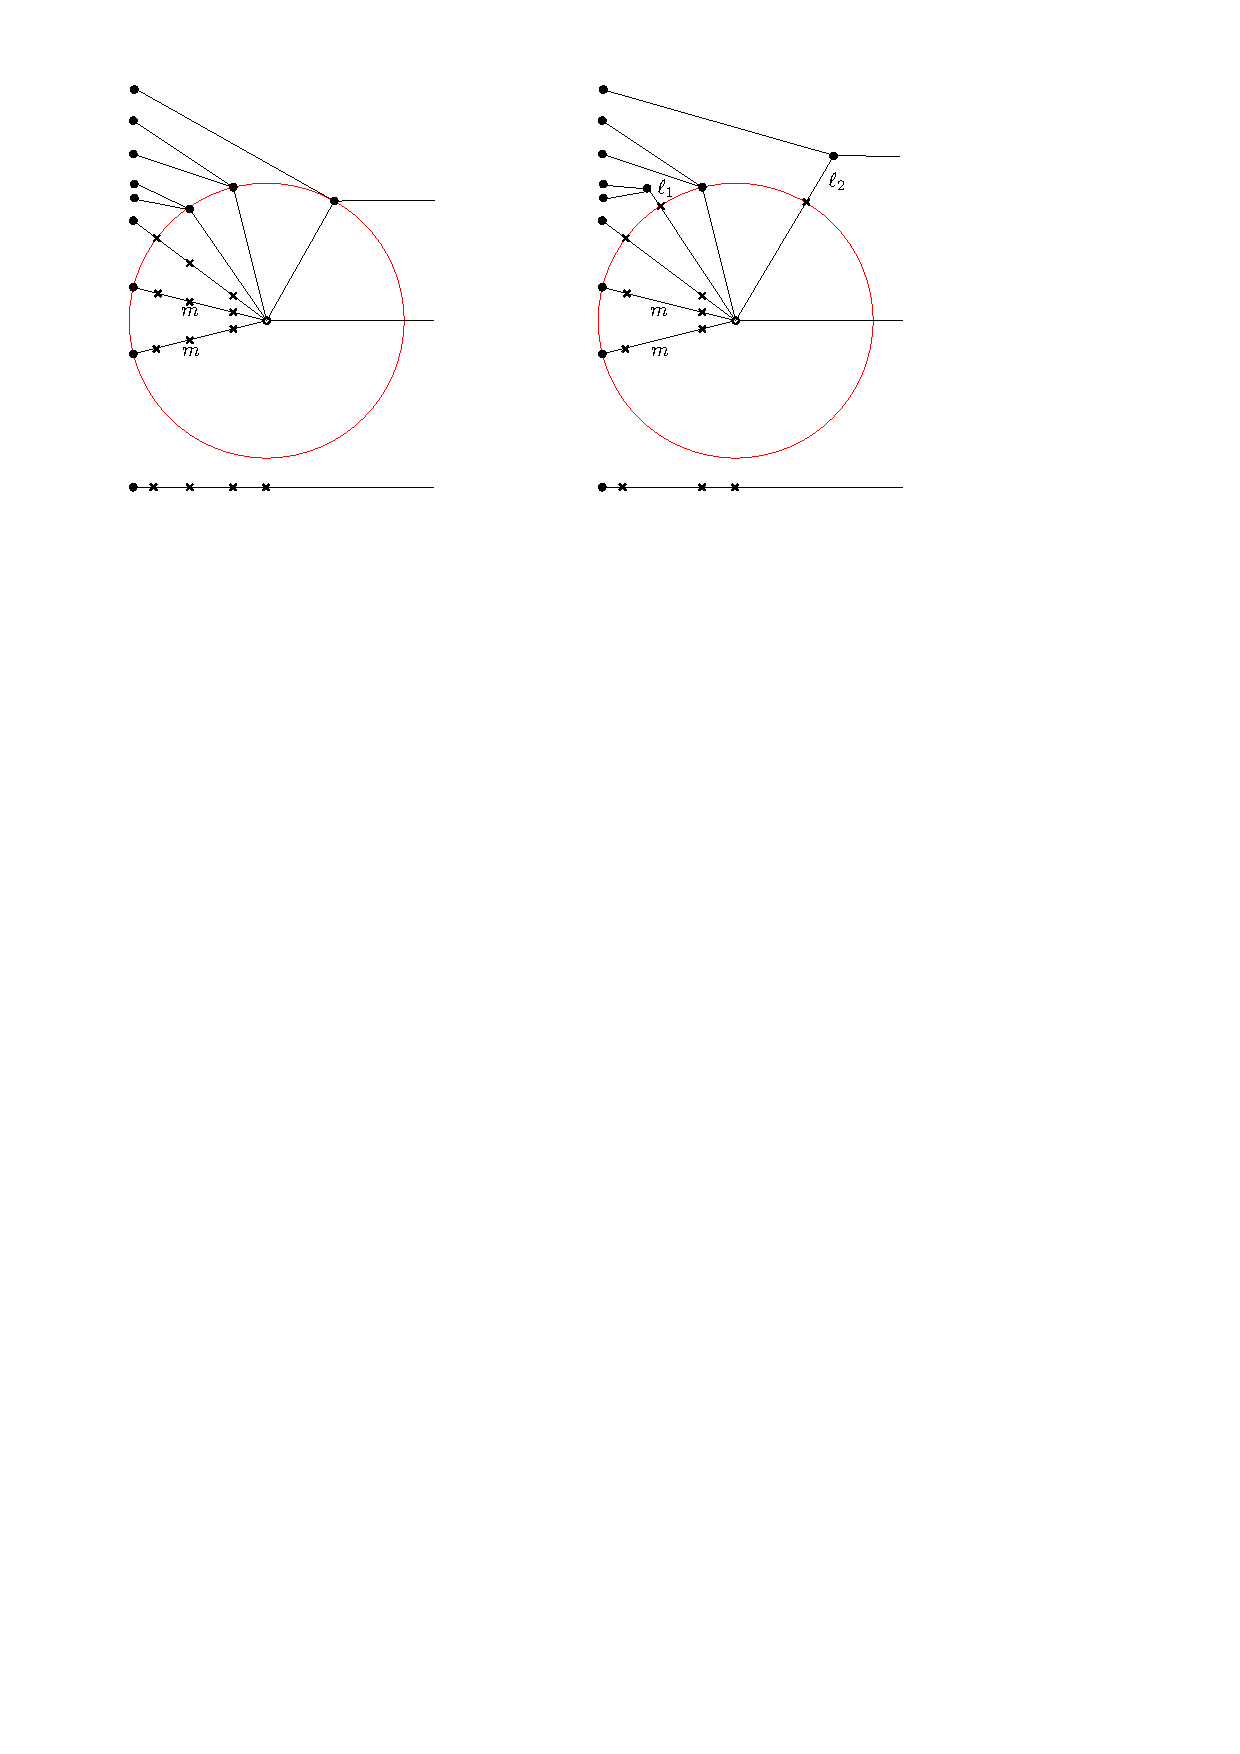
\includegraphics[scale=.3]{off_we_go}
\caption{Moving vertices off the circle creates new tropical parameters.}\label{fig:off_we_go}
\end{figure}

\subsubsection{$\Dcal$ from $\widetilde\Dcal$: first way}\label{subsection D from Dtilde} On $\widetilde\Dcal$ there is a tautological line bundle arising from the modular description of $\widetilde\VZ_{1,\alpha}(\PP^N|H,d)$, namely $\OO(\delta)$.


\begin{lemma}\label{lemma fibres of Odelta}
The fibre of $\OO(\delta)$ over a moduli point is naturally isomorphic to
\begin{equation*} T_{p}C^\prime \otimes T C_0\end{equation*}
where $C^\prime$ is any component of $C$ which lies on the radius, $p$ is the adjacent node which points towards the core, and $\TT_{C_0}$ is the universal tangent line bundle on the moduli space for $\sqC_0$.
\end{lemma}

\begin{proof}
Choose a component $C^\prime$ of the curve which lies on the circle. Then $\OO(\delta)$ is equal to the tensor product of tangent line bundles along the path of edges connecting $C^\prime$ to the core. However, this tensor product of line bundles is telescoping: any vertex which appears in the middle of the path will have an incoming and outgoing node, and since the vertex corresponds to a smooth rational curve these tangent spaces are naturally dual to each other~\cite[\S 2.2]{VZ}. Thus these factors cancel, and the result follows.
%Note that the final term on the right hand side is not given by $\TT_{q_i} C_0$ (where $q_i$ is the appropriate splitting node) but rather the tangent space to the core. 
\end{proof}
The content of Lemma \ref{lemma fibres of Odelta} is that the choice of point in the fibre of $\widetilde\Dcal \to \widetilde\Ecal$ provides a natural identification between the inward-pointing tangent spaces on the circle. This identification amounts to a specific linear dependence relation between the tangent vectors, which gives a point in the moduli space of attaching data for the corresponding elliptic singularity \cite[\S 2.2]{SMY2}. We may therefore express the factorisation condition in terms of the following natural morphism of vector bundles on $\widetilde\Dcal$:
\begin{equation*} \Sigma \operatorname{d}\!f \colon \OO(\delta)\otimes TC_0^\vee \to \ev_q^\st T H. \end{equation*}
Here $\Sigma \operatorname{d}\!f$ is defined by summing the images of the tangent vectors at the inward-pointing nodes on the circle, using the natural identification of each of these tangent spaces with $\OO(\delta)\otimes TC_0^\vee$ established above. \tred{We may assume it lands in $TH$ (rather than $T\PP^N$) thanks to Lemma \ref{lemma type C0 combinatorial types}.} This gives a section of the vector bundle
\begin{equation*} V = (\ev_q^\st TH) \otimes (TC_0) \otimes \OO(-\delta) \end{equation*}
which is transverse and whose vanishing locus coincides with $\Dcal$. Thus we obtain:
\begin{prop} \label{class of D} $[\Dcal] = \operatorname{e}(V) \cap [\widetilde\Dcal]$.\end{prop}
We claim that the class $\operatorname{e}(V)$ is tautological and computable. The only part which needs justification is $\OO(\delta)$. We claim that this can be obtained by pulling back a line bundle from $\Ecal$ and twisting by exceptional divisors.
\begin{lemma} For $i\in \{1,\ldots,r\}$ consider the line bundle
\begin{equation*} T_i = T_{q_i} C_i \otimes T_{q_i} C_0 \end{equation*}
on $\Ecal$, where $q_i$ is the splitting node. Then $\OO(\delta)$ is isomorphic to the pull-back of $T_i$ to $\widetilde\Dcal$ twisted by all exceptional divisors.\end{lemma}
We illustrate this lemma in the following example, which brings out the interplay between logarithmic moduli and blow-ups.
\begin{example}
Consider the locus $\Ecal$ given by $\sigma$ below, and the exceptional divisor $\widetilde\Dcal_\rho \subseteq \widetilde\Dcal$ given by $\rho$:
\begin{figure}[!htbp]
\begin{minipage}{0.3\textwidth}
\centering
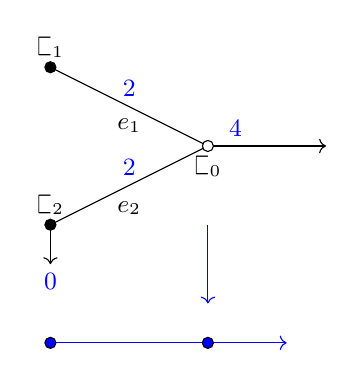
\begin{tikzpicture}
%\draw [red] plot [smooth cycle] coordinates {(0,-2) (-0.5,-1) (0,0) (1,0.5) (3,-1) (1,-2.5)};

\draw[fill=black] (0,0) circle[radius=2pt];
\draw (0,0) node[above]{\small$\sqC_1$};
\draw[fill=black] (0,0) -- (2,-1);
\draw (1,-0.95) node[above]{\small$e_1$};
\draw[color=blue] (1,-0.5) node[above]{\small$2$};

\draw[fill=black] (0,-2) circle[radius=2pt];
\draw (0,-2) node[above]{\small$\sqC_2$};

\draw[->] (0,-2) -- (0,-2.5);
\draw[color=blue] (0,-2.5) node[below]{\small$0$};

\draw[fill=black] (0,-2) -- (2,-1);
\draw (1,-2) node[above]{\small$e_2$};
\draw[color=blue] (1,-1.5) node[above]{\small$2$};

\draw[fill=black,->] (2,-1) -- (3.5,-1);
\draw[color=blue] (2.35,-1) node[above]{\small$4$};

\draw[fill=white] (2,-1) circle[radius=2pt];
\draw (2,-1) node[below]{\small$\sqC_0$};

\draw[color=blue,->] (2,-2) -- (2,-3);

\draw[color=blue,->] (0,-3.5) -- (3,-3.5);
\draw[fill=blue] (0,-3.5) circle[radius=2pt];
\draw[fill=blue] (2,-3.5) circle[radius=2pt];
\end{tikzpicture}
\caption{$\sigma$}
\end{minipage}\hfill
\begin{minipage}{0.7\textwidth}
\centering
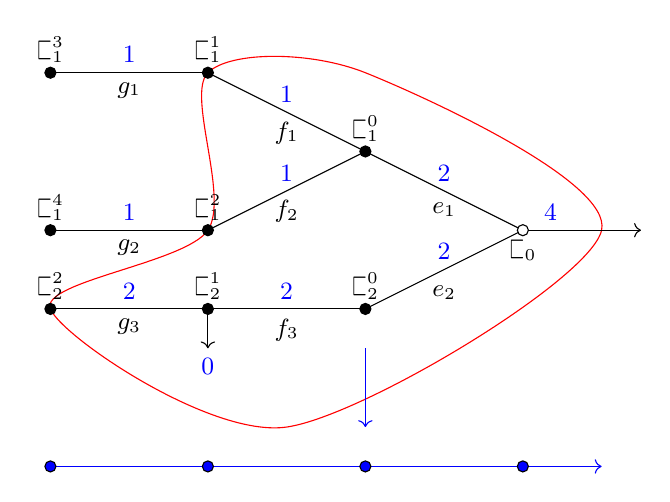
\begin{tikzpicture}
\draw [red] plot [smooth cycle] coordinates {(-4,-2) (-2,-1) (-2,1) (0,1) (3,-1) (-1,-3.5)};

\draw[fill=black] (0,0) circle[radius=2pt];
\draw (0,0) node[above]{\small$\sqC_1^0$};
\draw[fill=black] (0,0) -- (2,-1);
\draw (1,-0.95) node[above]{\small$e_1$};
\draw[color=blue] (1,-0.5) node[above]{\small$2$};

\draw[fill=black] (0,-2) circle[radius=2pt];
\draw (0,-2) node[above]{\small$\sqC_2^0$};
\draw[fill=black] (0,-2) -- (2,-1);
\draw (1,-2) node[above]{\small$e_2$};
\draw[color=blue] (1,-1.5) node[above]{\small$2$};

\draw[fill=black,->] (2,-1) -- (3.5,-1);
\draw[color=blue] (2.35,-1) node[above]{\small$4$};

\draw[fill=white] (2,-1) circle[radius=2pt];
\draw (2,-1) node[below]{\small$\sqC_0$};

\draw (-2,1) -- (0,0);
\draw[fill=black] (-2,1) circle[radius=2pt];
\draw (-2,1) node[above]{\small$\sqC_1^1$};
\draw (-1,0.5) node[below]{\small$f_1$};
\draw[color=blue] (-1,0.5) node[above]{\small$1$};

\draw (-2,1) -- (-4,1);
\draw[fill=black] (-4,1) circle[radius=2pt];
\draw (-4,1) node[above]{\small$\sqC_1^3$};
\draw (-3,1) node[below]{\small$g_1$};
\draw[color=blue] (-3,1) node[above]{\small$1$};

\draw (-2,-1) -- (0,0);
\draw[fill=black] (-2,-1) circle[radius=2pt];
\draw (-2,-1) node[above]{\small$\sqC_1^2$};
\draw (-1,-0.5) node[below]{\small$f_2$};
\draw[color=blue] (-1,-0.5) node[above]{\small$1$};

\draw (-2,-1) -- (-4,-1);
\draw[fill=black] (-4,-1) circle[radius=2pt];
\draw (-4,-1) node[above]{\small$\sqC_1^4$};
\draw (-3,-1) node[below]{\small$g_2$};
\draw[color=blue] (-3,-1) node[above]{\small$1$};

\draw (0,-2) -- (-2,-2);
\draw[fill=black] (-2,-2) circle[radius=2pt];
\draw (-2,-2) node[above]{\small$\sqC_2^1$};
\draw (-1,-2) node[below]{\small$f_3$};
\draw[color=blue] (-1,-2) node[above]{\small$2$};
\draw[->] (-2,-2) -- (-2,-2.5);
\draw[color=blue] (-2,-2.5) node[below]{\small$0$};

\draw (-2,-2) -- (-4,-2);
\draw[fill=black] (-4,-2) circle[radius=2pt];
\draw (-4,-2) node[above]{\small$\sqC_2^2$};
\draw (-3,-2) node[below]{\small$g_3$};
\draw[color=blue] (-3,-2) node[above]{\small$2$};

\draw[color=blue,->] (0,-2.5) -- (0,-3.5);

\draw[color=blue,->] (-4,-4) -- (3,-4);
\draw[fill=blue] (0,-4) circle[radius=2pt];
\draw[fill=blue] (2,-4) circle[radius=2pt];
\draw[fill=blue] (-2,-4) circle[radius=2pt];
\draw[fill=blue] (-4,-4) circle[radius=2pt];
\end{tikzpicture}
\caption{$\rho$}
\end{minipage}
\end{figure}

On the cone $\rho$ we have the following tropical continuity equations
\begin{align*}
e:=e_1 = e_2, \qquad f:=f_1 = f_2 = 2f_3, \qquad g:=g_1 = g_2 = 2g_3
\end{align*}
together with the equation imposed by the choice of alignment:
\begin{align*} e_1 + f_1 = e_2 + f_3 + g_3 \qquad (\Longleftrightarrow f = g).
\end{align*}
From now on we use the same symbol to denote an edge length and the corresponding node on $\widetilde\Dcal_\rho$. On this locus we have line bundles pulled back from $\Ecal$
\begin{align*} T_1 & = T_{e_1} C_1^0 \otimes T_{e_1} C_0 \\
T_2 & = T_{e_2} C_2^0 \otimes T_{e_2} C_0\end{align*}
as well as the logarithmic line bundle
\begin{equation*} \OO(\delta) = T_{f_1} C_1^1 \otimes T_{e_1} C_0 = T_{f_2} C_1^2 \otimes T_{e_1} C_0 = T_{g_3} C_2^2 \otimes T_{e_2}C_0 
\end{equation*}
where the identifications follow from Lemma \ref{lemma fibres of Odelta}. We claim that: 
\begin{equation} \label{Odelta eqn} \OO(\delta) = T_1\otimes \OO(\widetilde\Dcal_\rho) = T_2 \otimes \OO(\widetilde\Dcal_\rho).\end{equation}
Notice that $\OO(\widetilde\Dcal_\rho) = \OO(f)=\OO(g)$. Thus we have
\begin{align*} T_1 \otimes \OO(\widetilde\Dcal_\rho) & = \OO(f_1) \otimes T_{e_1} C_1^0 \otimes T_{e_1}C_0 \\
& = T_{f_1}C_1^1 \otimes T_{f_1} C_1^0 \otimes T_{e_1} C_1^0 \otimes T_{e_1}C_0  \\
& = T_{f_1}C_1^1\otimes T_{e_1}C_0 \qquad (= \OO(\delta))
\end{align*}
where in the last line we have used the same telescoping trick $\TT_{f_1}C_1^0 \otimes \TT_{e_1} C_1^0 = \OO$ used in the proof of Lemma \ref{lemma fibres of Odelta}. On the other hand, for $T_2$ we may write $f=f/2 + g/2=f_3+g_3$ in order to obtain:
\begin{equation*} T_2 \otimes \OO(\widetilde\Dcal_\rho) = \OO(g_3) \otimes \OO(f_3) \otimes T_{e_2} C_2^0 \otimes T_{e_2} C_0 = T_{g_3}C_2^2 \otimes T_{e_2}C_0 = \OO(\delta) \end{equation*}
where we have used the same telescoping trick. Thus we have proven \eqref{Odelta eqn}. This observation generalises, giving a precise relation between the intrinsically-defined line bundle $\OO(\delta)$ on $\widetilde\Dcal$ (which we use to impose the factorisation condition) and the the line bundles $T_i$ pulled back from $\Ecal$. This allows us to express the Chern classes of $\OO(\delta)$ (and hence $V$) in terms of pull-backs of tautological classes from $\Ecal$ and boundary strata on $\widetilde\Dcal$, which is sufficient in order to compute integrals.
\end{example}


\subsubsection{$\Dcal$ from $\widetilde\Dcal$: second way} To establish a more direct connection with the geometry of the fibre product \eqref{IIIa fibre product}, recall that $\widetilde\Ecal$ has been built as an explicit modification of a finite cover of \eqref{IIIa fibre product}. For every $v\in\{\sqC_1,\ldots,\sqC_r\}$ - with the convention established at the end of Lemma \ref{lem:generic_proj_bundle} -, on $\widetilde\Ecal$ it makes sense to consider the line bundle $\OO(\delta_v)$ associated to a shortest path from the core to the circle in the $v$-direction. Construct $\mathcal P=\PP_{\widetilde\Ecal}(\bigoplus_{v\in \{\sqC_1,\ldots,\sqC_r\}}\OO(\delta_v))$; since $\sqC_1,\ldots,\sqC_r$ are always ordered on $\widetilde \Dcal$ (they may lie on the circle, be the first component off the circle, or degenerate and lie in the strict interior), there is a morphism $\widetilde \Dcal\to\mathcal P$ lifting $\widetilde \Dcal\to\widetilde\Ecal$. Consider the map of vector bundles on $\mathcal P$:
\[ \OO_{\mathcal P}(-1)\to p^*(\bigoplus_{v\in \{\sqC_1,\ldots,\sqC_r\}}\OO(\delta_v))\xrightarrow{\sum\operatorname{d}f}\ev_{C_0}^*TH.\]

The composite, regarded as a section $s$ of $G=\OO_{\mathcal P}(1)\otimes \operatorname{ev}_{C_0}^*(TH)$, vanishes precisely where $f$ factors through the elliptic singularity determined by the point in the fiber of $p$. Generically on $\widetilde\Ecal$, this is exactly what we are after - compare with Lemma \ref{lem:generic_proj_bundle}. On the boundary, though, it may happen that a simultaneous degeneration in the base and the fiber makes this factorisation trivial, in the sense that $\bar f$ would be constant on all the branches of the elliptic singularity.

\begin{lemma}
 For every $\Lambda_B\subseteq \{\sqC_1,\ldots,\sqC_r\}$ and $\Lambda_F=\{\sqC_1,\ldots,\sqC_r\}\setminus \Lambda_B$, $s$ vanishes along the loci where the factors corresponding to $\Lambda_B$ in $\widetilde \Ecal$ degenerate so that $f_i\colon C_i\to\PP^N$ is constant in a neighbourhood of $q_i$, and the fiber coordinates $(\lambda_j)_{j\in\Lambda_F}$ along $p\colon\mathcal P\to\widetilde \Ecal$ are set to be $0$.
\end{lemma}
Call these loci $\Xi_i,i\in I$ (compare with \cite[\S 3.2]{VZ} for an analogous phenomenon in the non-relative case); clearly, they may be in excess with respect to the expected codimension of $V(s)$, that is $N-1$. These loci are logarithmic substrata; therefore, there exists a logarithmic blow-up that principalizes them. We claim that $\widetilde\Dcal$ is (possibly a refinement of) such a blow-up. 
\begin{lemma}
 The pullback of $\Xi_i$ is principal in $\widetilde\Dcal$.
\end{lemma}
\begin{proof}
 Let us analyse the ideal of $\Xi_i$: it is generated by
 \begin{enumerate}[leftmargin=.5 cm]
  \item equations on $\widetilde\Ecal$ cutting the locus where $C_i$ degenerates so that $f_i$ is constant on a neighbourhood of $q_i$, $i\in \Lambda_B$: these correspond to the tropical functions $\delta_i-\operatorname{dist}(q_i,\circ)$;
  \item equations on the fiber of $p$ for the linear subspace corresponding to $j\in \Lambda_F$: tropically, these correspond to the $\ell_j$ discussed in Lemma Lemma \ref{lem:generic_proj_bundle}.
 \end{enumerate}
By construction, on $\widetilde \Dcal$ it is always possible to tell which of these tropical lengths is the shortest (the circle we have drawn on $\Xi$ is degenerate - it passes through no vertex of positive horizontal degree -, therefore we need to decide for a strictly larger circle in order to lift to $\widetilde D$), which corresponds to principalising the ideal (see Figure \ref{fig:principalisation}).
\end{proof}

\begin{figure}
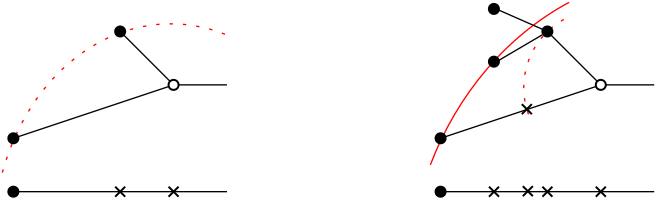
\includegraphics[scale=.5]{principalisation}
\caption{On the left, a generic point of $\mathcal P$. On the right, a point of $\Xi$. The dotted circle is the one we draw on $\mathcal P$. The continuous circle represents one of the possible choices of $\delta$ enlarging the dotted one (a stratum of $\widetilde\Dcal$).}\label{fig:principalisation}
\end{figure}

Finally, on $\widetilde\Dcal$ (or, in fact, on an intermediate blow-up $\widetilde{\mathcal P}\to\mathcal P$) there are exceptional divisors $\widetilde \Xi_i$ corresponding to $\Xi_i$ in $\mathcal P$. Since the $\Xi_i$ exhaust all the excess-dimensional components of the vanishing locus of $s\in\Gamma(\mathcal P,G)$, the latter induces a section $\tilde s\in\Gamma(\widetilde\Dcal,G(-\sum_i\widetilde\Xi_i))$ by pullback and twisting, whose vanishing locus is dimensionally transverse to the boundary, and whose open part coincides with the generic point of $\Dcal$, therefore $V(\tilde s)=\Dcal$.

Expressing the pushforward of the Chern classes of $\OO_F(1)$ and $\OO(\widetilde\Xi_i)$ in terms of tautological classes on the fiber product underlying $\Ecal$, we get:
\begin{cor}
 After pushforward to $\Ecal$, the contribution of $\Dcal$ to the invariants can be computed in terms of tautological integrals on moduli spaces of maps with lower numerics.
\end{cor}

\subsection{Recursion for general $(X,Y)$}\label{section recursion for general pair} Now let $(X,Y)$ be a general smooth very ample pair. In \S \ref{} we studied the moduli space $\VZ_{1,\alpha}(X|Y,\beta)$ of centrally aligned maps to $(X,Y)$ and equipped it with a virtual fundamental class by diagonal pull-back from $\VZ_{1,\alpha}(\PP^N|H,d)$.

This construction of the virtual fundamental class means that once we have established a recursion formula for $(\PP^N,H)$, it immediately pulls back to give a recursion formula for $(X,Y)$. To be more precise, Theorem \ref{theorem recursion} holds \emph{mutatis mutandis}, with the same values of $\lambda_\Dcal$. The computation of the splitting orders is exactly the same, and the recursive description of the boundary strata pulls back to give an entirely analogous description on $\VZ_{1,\alpha}(X|Y,\beta)$.


\section{Quantum Lefschetz algorithm}\label{section recursion algorithm}
Consider a smooth pair $(X,Y)$ with $Y$ very ample, and let $\mathbb{P}$ be the projective bundle $\mathbb{P}=\PP_Y(\operatorname{N}_{Y|X} \oplus\OO_Y)$. We assume that the genus zero and reduced genus one Gromov--Witten theories of $X$ are known. From this starting data, we will apply our recursion formula to compute:
\begin{enumerate}
\item the genus one \textbf{reduced restricted absolute Gromov--Witten theory} of $Y$;
\item the genus one \textbf{reduced relative Gromov--Witten theory} of the pair $(X,Y)$;
\item the genus one \textbf{reduced rubber theory} of $\mathbb{P}$.
\end{enumerate}

\subsection{Reduced absolute, relative and rubber invariants} To be precise: by a reduced invariant of $Y$ we mean an integral over $\VZ_{1,n}(Y,\beta)$ of products of pullbacks of evaluation and psi classes along morphisms which forget a subset $S$ of the marked points (taking $S=\emptyset$ gives the ordinary evaluation and psi classes). Here the evaluation maps are viewed as mapping into $X$ (hence the adjective ``restricted''). Reduced relative invariants of $(X,Y)$ are defined in the same way, except now the forgetful morphism maps into a space of absolute maps:
\begin{equation*} \fgt_S \colon \VZ_{1,\alpha}(X|Y,\beta) \to \VZ_{1,m-\#S}(X,\beta).\end{equation*}
In particular, all the psi classes which we consider are \emph{collapsed psi classes}, meaning that they are relative cotangent line classes for the corresponding collapsed stable map. Note that, unlike in the absolute case, in the relative case it may well be the case that the entire insertion is pulled back along a single forgetful map $\fgt_S$. The reduced rubber invariants of $\mathbb{P}$ are defined similarly (again using collapsed psi classes).

The systems of invariants defined above are equivalent to the classical systems of invariants (which do not use forgetful morphisms) by well-known topological recursion relations.

\subsection{Fictitious and true markings} The recursion procedure is rather delicate. Roughly speaking, we will induct on the degree (meaning $Y\cdot\beta$), number of marked points and total tangency. To get the correct notion of number of markings and total tangency in  the relative setting, we introduce the concept of \textbf{fictitious markings}. Consider a moduli space $\VZ_{1,\alpha}(X|Y,\beta)$ of reduced relative stable maps and a corresponding integrand $\gamma$. We let $F \subseteq \{1,\ldots,m\}$ be the maximal subset of marked points such that:
\begin{enumerate}
\item $\alpha_i = 1$ for all $i \in F$;
\item the entire integrand $\gamma$ is pulled back along $\fgt_F$.
\end{enumerate}
This subset is uniquely determined, and its elements are referred to as \textbf{fictitious markings}. Markings which are not fictitious are referred to as \textbf{true}. When inducting on relative invariants we will always be interested in the number of true markings (as opposed to the total number of markings) and the true tangency
\begin{equation*} \sum_{i \not\in F} \alpha_i \leq d=Y\cdot \beta \end{equation*}
as opposed to the total tangency, which is always $d$. This formalises the idea that relative invariants with non-maximal tangency $t<d$ can be obtained by adding $d-t$ fictitious markings of tangency $1$; see \cite[Lemma 1.15(i)]{Ga}.

\subsection{Structure of the recursion} Given the genus-zero Gromov--Witten theory of $X$, the arguments of \cite{Ga} give an effective algorithm to reconstruct the genus-zero theories of $Y$ and $(X,Y)$; moreover, the genus-zero rubber theory of $\mathbb{P}$ is identical to the genus-zero theory of $Y$ \cite{GathmannThesis}. Thus we may assume that all genus-zero data is known. We assume in addition that we know the genus one reduced theory of $X$. The structure of the recursion is then as follows:

\begin{algorithm}
\DontPrintSemicolon
\For{$d \geq 0$}{
\For{$n \geq 0$}{
\For{$t \geq 0$\medskip}{
\textbf{\, Step 1: } Compute forgetful relative invariants of $(X,Y)$ (degree~$d$, $n+1$ true markings, true tangency $t$); see below.
}
\medskip \textbf{Step 2: } Compute absolute invariants of $Y$ (degree $d$, $n$ markings).\;
\For{$t \geq 0$\medskip}{
\textbf{\, Step 3: } Compute relative invariants of $(X,Y)$ (degree $d$, $n$ true markings, true tangency $t$).\;
}
}
\For{$n \geq 0$\medskip}{
\For{$m \geq 0$\medskip}{
\textbf{\, Step 4: } Compute rubber invariants of $\mathbb{P}$ (degree $d$, $n$ relative markings, $m$ non-relative markings).
}
}
}
\end{algorithm}
\noindent Although the loops involving $d, n$ and $m$ have infinite length, in order to compute any single invariant it is only necessarily to iterate the preceding loops for a finite amount of time. A \textbf{forgetful relative invariant} of $(X,Y)$ is by definition a reduced relative invariant with a marked point $x_0$ such that all of the insertions are pulled back along $\fgt_{x_0}$. In our recursion, we first deal with this special class of relative invariants (with $n+1$ true markings), before computing the absolute invariants (with $n$ markings) and then returning to compute all of the relative invariants (with $n$ true markings). This need to treat separately a particular subclass of the relative invariants is an inescapable feature of the genus one recursion.

The base terms of the recursion all have $d=0$ and as such are easy to compute: the relative invariants of $(X,Y)$ are nothing but absolute invariants of $X$ and the absolute invariants of $Y$ are given by obstruction bundle integrals over Deligne--Mumford spaces. The rubber invariants of $\mathbb{P}$ in degree zero are given by integrals over the main component of the double ramification cycle; this can likewise be computed as an integral over Deligne--Mumford space, by correcting the formula for the ordinary double ramification cycle \cite{Hain,JPPZ} by the obvious contribution from the boundary irreducible component (the observation which makes this easy to do in genus one is that the rubber moduli space is pure-dimensional, so that the virtual class is simply the sum of the fundamental classes of the irreducible components). We will now explain how to perform each of the four inductive steps outlined above.

\begin{notation}Given tuples $\mathbf{a}=(a_1,\ldots,a_n)$ and $\mathbf{b}=(b_1,\ldots,b_n)$, we say that $\mathbf{a}<\mathbf{b}$ if there exists an $i \in \{1,\ldots,n\}$ such that $a_j = b_j$ for $j < i$ and $a_i < b_i$.\end{notation}

\subsection*{Step 1} Suppose we are given a forgetful relative invariant to compute. That is, we have a relative space $\VZ_{1,\alpha}(X|Y,\beta)$ of degree $d$, with $n+1$ true markings and true tangency $t$, and a marking $x_0$ such that the insertion $\gamma$ is pulled back along $\fgt_{x_0}$. We assume inductively that every absolute, relative and rubber invariant with $(d^\prime,n^\prime) < (d,n)$ is known, and also that every forgetful relative invariant with $(d^\prime,n^\prime,t^\prime) < (d,n+1,t)$ is known. Choose a true marking $x_1$ with $\alpha_1 \geq 1$ and consider the space:
\begin{equation*} \VZ_{1,(\alpha-e_1) \cup (1)}(X|Y,\beta). \end{equation*}
Denote the newly-introduced marking by $y$ and consider the integrand $\tilde\gamma$ obtained from $\gamma$ by introducing $\fgt_y^\st$ everywhere. Applying our recursion formula to $x_1$, we obtain:
\begin{equation}\label{step 1 recursion}\left( (\alpha_1-1)\psi_1 + \ev_1^\st Y\right) \tilde\gamma \cap [\VZ_{1,(\alpha-e_1) \cup (1)}(X|Y,\beta)] = \tilde\gamma \cap [\Dcal(1)].\end{equation}
Let us first examine the left-hand side. The class $\psi_1$ differs from $\fgt_y^\st \psi_1$ by the locus where $x_1$ and $y$ are contained on a contracted rational bubble. This locus consists of reduced relative stable maps of the form \medskip

\begin{center}
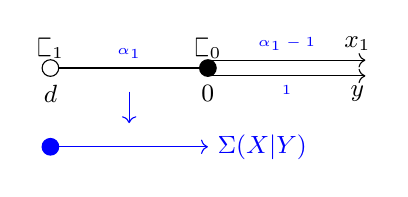
\begin{tikzpicture}[scale=1]
%edge
\draw (0,0) to (2,0);
\draw [color=blue] (1,0) node[above]{\tiny$\alpha_1$};

%C_1
\draw [fill=white] (0,0) circle[radius=3pt];
\draw (0,-0.1) node[below]{\small$d$};
\draw (0,0) node[above]{\small$\sqC_1$};

%C_0
\draw [fill=black] (2,0) circle[radius=3pt];
\draw (2,-0.1) node[below]{\small$0$};
\draw (2,0) node[above]{\small$\sqC_0$};

%x_1
\draw [->] (2,0.1) -- (4,0.1);
\draw (3.9,0.1) node[above]{\small$x_1$};
\draw [color=blue](3,0.1) node[above]{\tiny$\alpha_1-1$};

%y
\draw [->] (2,-0.1) -- (4,-0.1);
\draw (3.9,-0.1) node[below]{\small$y$};
\draw [color=blue] (3,-0.1) node[below]{\tiny$1$};

%down arrow
\draw [color=blue,->] (1,-0.3) -- (1,-0.7);

%target
\draw [color=blue,->] (0,-1) to (2,-1);
\draw [fill=blue,color=blue] (0,-1) circle[radius=3pt];
\draw [color=blue] (2,-1) node[right]{\small$\Sigma(X|Y)$};
\end{tikzpicture}
\end{center}
% Algebro-geometric picture; replaced by tropical picture.
%%%%%%%%%%%%%%%%%%%%%%%%%%%%%%%%%%%%%%%%%%%%%%%%%%%%%%%%%%%
\begin{comment}
\begin{center}
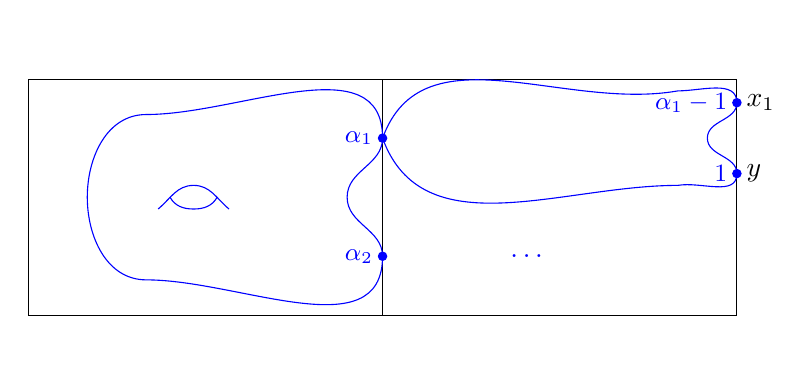
\begin{tikzpicture}[scale=1.5]
%Draw target
\draw (0,0) -- (3,0) -- (3,2) -- (0,2) -- (0,0);
\draw (3,0) -- (6,0) -- (6,2) -- (3,2) -- (3,0);

%Draw genus one curve on left-hand side
\draw [blue] (3,0.5) to [out=90,in=270] (2.7,1) to [out=90,in=270] (3,1.5) to [out=90,in=0] (1,1.7) to [out=180,in=90] (0.5,1) to [out=270,in=180] (1,0.3) to [out=0,in=270] (3,0.5);
\draw [blue] (1.1,0.9) to [out=40, in=180] (1.4,1.1) to [out=0,in=140] (1.7,0.9);
\draw [blue] (1.2,1) to [out=300, in=180] (1.4,0.9) to [out=0,in=240] (1.6,1);

%Draw nodal blobs
\draw [fill=blue,color=blue] (3,0.5) circle[radius=1pt];
\draw [color=blue] (3,0.5) node[left]{\small$\alpha_2$};
\draw [fill=blue,color=blue] (3,1.5) circle[radius=1pt];
\draw [color=blue] (3,1.5) node[left]{\small$\alpha_1$};
%Draw rational bubble with x_1 and y
\draw [blue] (3,1.5) to [out=70,in=190] (5.5,1.9) to [out=0,in=90] (6,1.8) to [out=270,in=90] (5.75,1.5) to [out=270,in=90] (6,1.2) to [out=270,in=10] (5.5,1.1) to [out=180,in=290] (3,1.5);

%Draw right-hand markings
\draw [fill=blue,color=blue] (6,1.8) circle[radius=1pt];
\draw [color=blue] (6,1.8) node[left]{\small{$\alpha_1-1$}};
\draw (6,1.8) node[right]{$x_1$};
\draw [fill=blue,color=blue] (6,1.2) circle[radius=1pt];
\draw [color=blue] (6,1.2) node[left]{\small{$1$}};
\draw (6,1.2) node[right]{$y$};

%Draw ldots
\draw [color=blue] (4,0.5) node[right]{$\ldots$};
\end{tikzpicture}
\end{center}
\end{comment}
%%%%%%%%%%%%%%%%%%%%%%%%%%%%%%%%%%%%%%%%%%%%%%%%%%%%%%%%%
with all other marked points contained on $\sqC_1$. This is isomorphic to $\VZ_{1,\alpha}(X|Y,\beta)$ and when we restrict $\tilde\gamma$ to this locus we obtain precisely the class $\gamma$ which we started with. Thus the left-hand side of \eqref{step 1 recursion} may be written as
\begin{equation*} (\alpha_1-1) I + \fgt_y^\st \left( (\alpha_1-1)\psi_1 + \ev_1^\st Y\right)  \tilde\gamma \cap [\VZ_{1,(\alpha-e_1)\cup(1)}(X|Y,\beta)]\end{equation*}
where $I$ is the invariant we are trying to compute. The second term is a forgetful relative invariant with the same degree and number of true markings (since $y$ is fictitious), and strictly smaller true tangency; hence it is recursively known. We now examine the right-hand side of \eqref{step 1 recursion}. Recall that all of the genus zero data has already been computed, so we only need to focus on the genus one pieces. First consider the type $A$ loci. The genus one piece has strictly smaller degree (and hence is recursively known) exept in the following situation (with some stable distribution of the remaining markings):
\begin{center}
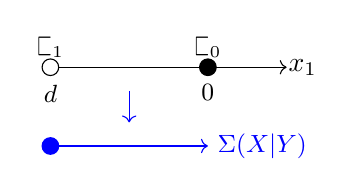
\begin{tikzpicture}[scale=1]
\draw (0,0) to (2,0);
\draw [fill=white] (0,0) circle[radius=3pt];
\draw (0,-0.1) node[below]{\small$d$};
\draw (0,0) node[above]{\small$\sqC_1$};
\draw [fill=black] (2,0) circle[radius=3pt];
\draw (2,-0.1) node[below]{\small$0$};
\draw (2,0) node[above]{\small$\sqC_0$};
\draw [->] (2,0) -- (3,0);
\draw (2.9,0) node[right]{$x_1$};

\draw [color=blue,->] (1,-0.3) -- (1,-0.7);

\draw [color=blue,->] (0,-1) to (2,-1);
\draw [fill=blue,color=blue] (0,-1) circle[radius=3pt];
\draw [color=blue] (2,-1) node[right]{\small$\Sigma(X|Y)$};
\end{tikzpicture}
\end{center}
In this situation, $C_1$ contains at most $n+1$ true markings. If it has $n-1$ or fewer, than it is known recursively. If it has exactly $n$ this means that $C_0$ contains exactly one true marking (besides $x_1$, which may be true or fictitious). We claim that in this situation we must have $y \in C_1$, since otherwise we would have a moduli space for $C_0$ given by $\ol\Mcal_{0,k}$ with $k \geq 4$, and  applying the projection formula with $\fgt_y$ we would conclude that the contribution is zero. Thus we have $y \in C_1$, and so the genus one contribution is a forgetful relative invariant with $n$ true markings, and hence is recursively known.

Finally, if $C_1$ contains exactly $n+1$ true markings, then the only additional markings on $C_0$ are fictitious, and by the same argument as in the previous paragraph there can only be one. Thus for each fictitious marked point we obtain a locus isomorphic to $\VZ_{1,\alpha}(X|Y,\beta)$ and $\tilde\gamma$ restricts to $\gamma$ here (from the point of view of computing invariants, the fictitious marked points are indistinguishable, meaning that the contributions are all the same). Thus for each fictitious marked point (of which there is at least one, namely $y$) we get a contribution of $\alpha_1 I$ to the right-hand side of \eqref{step 1 recursion}.

The contributions of the type $B$ loci only involve genus zero data and hence are known. The contributions of the type $C^0$ loci are determined by genus zero data and tautological integrals on Deligne--Mumford space, hence are also known. It remains to consider type $C^+$ loci. If the degree of the genus one piece is less than $d$ then we have a rubber invariant of strictly smaller degree. The only other possibility is that the entire curve is mapped into the divisor. In this case we may apply the projection formula with $\fgt_y$ to identify this with an integral over $\VZ_{1,m}(Y,\beta)$ for some (possibly large) number $m$ of marked points. But by assumption there is another marked point $x_0$ with all of the insertions pulled back along $\fgt_{x_0}$, so a further application of the projection formula shows that this contribution vanishes. To conclude, we may rearrange \eqref{step 1 recursion} to obtain an expression of the form
\begin{equation*} \lambda I = \text{recursively known terms} \end{equation*}
where $\lambda$ is an explicit scalar which is always nonzero; we have thus determined $I$, which completes Step 1.

\subsection*{Step 2} Consider now the absolute space $\VZ_{1,n}(Y,\beta)$ with an insertion $\gamma$, and suppose inductively that we have computed all forgetful relative invariants with $(d^\prime,n^\prime) \leq (d,n+1)$, all relative invariants and absolute invariants with $(d^\prime,n^\prime) < (d,n)$, and all special rubber invariants with $d^\prime < d$. Consider the following moduli space with $n+1$ markings:
\begin{equation*} \VZ_{1,(d,0,\ldots,0)}(X|Y,\beta). \end{equation*}
Let $x_0$ denote the relative marking and consider the integrand $\tilde\gamma$ obtained from $\gamma$ by introducing $\fgt^\st_{x_0}$ everywhere. Now recurse at $x_1$ to obtain:
\begin{equation}\label{step 2 recursion} \ev_1^\st Y \cdot \tilde\gamma \cap [\VZ_{1,(d,0,\ldots,0)}(X|Y,\beta)] = \tilde\gamma\cap[\Dcal(1)].\end{equation}
The left-hand side is a forgetful relative invariant of degree $d$ and $\leq n+1$ true markings, and so has already been computed. For the right-hand side, let us begin with loci of type $A$. The genus one contributions from each loci have $(d^\prime,n^\prime) < (d,n)$ except in the following case
\begin{center}
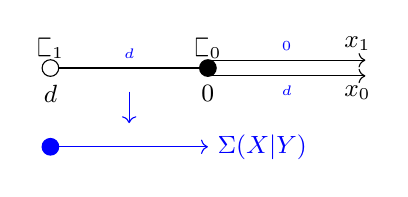
\begin{tikzpicture}[scale=1]
%edge
\draw (0,0) to (2,0);
\draw [color=blue] (1,0) node[above]{\tiny$d$};

%C_1
\draw [fill=white] (0,0) circle[radius=3pt];
\draw (0,-0.1) node[below]{\small$d$};
\draw (0,0) node[above]{\small$\sqC_1$};

%C_0
\draw [fill=black] (2,0) circle[radius=3pt];
\draw (2,-0.1) node[below]{\small$0$};
\draw (2,0) node[above]{\small$\sqC_0$};

%x_1
\draw [->] (2,0.1) -- (4,0.1);
\draw (3.9,0.1) node[above]{\small$x_1$};
\draw [color=blue](3,0.1) node[above]{\tiny$0$};

%y
\draw [->] (2,-0.1) -- (4,-0.1);
\draw (3.9,-0.1) node[below]{\small$x_0$};
\draw [color=blue] (3,-0.1) node[below]{\tiny$d$};

%down arrow
\draw [color=blue,->] (1,-0.3) -- (1,-0.7);

%target
\draw [color=blue,->] (0,-1) to (2,-1);
\draw [fill=blue,color=blue] (0,-1) circle[radius=3pt];
\draw [color=blue] (2,-1) node[right]{\small$\Sigma(X|Y)$};
\end{tikzpicture}
\end{center}
which gives a contribution of
\begin{equation*} d\cdot \gamma \cap [\VZ_{1,(d,\underbrace{0,\ldots,0}_{n-1})}(X|Y,\beta)] \footnote{(Navid) Fix formatting}\end{equation*}
to the right-hand side of \eqref{step 2 recursion}. Here $\gamma$ is the insertion we started with; the difference is that we are now considering relative maps to $(X,Y)$ with maximal tangency at $x_1$, rather than absolute maps to $Y$. The type $B$ and $C^0$ loci are recursively determined as in Step~1, and similarly the type $C^+$ loci are recursively determined except for the locus where the entire curve is mapped into the divisor. On this locus we may apply $\fgt_{x_0}$ and identify the contribution with
\begin{equation*} d^2 \cdot \gamma \cap [\VZ_{1,n}(Y,\beta)] = d^2 \cdot I \end{equation*}
where $I$ is the invariant we are trying to compute. Putting this all together, we obtain
\begin{equation}\label{step 2 recursion 2} I = (-\gamma/d) \cap [\VZ_{1,(d,\underbrace{0,\ldots,0}_{n-1})}(X|Y,\beta)] + \text{recursively known terms} \end{equation}
where on the right-hand side there are $n-1$ non-relative markings $x_2,\ldots,x_n$, and a relative marking $x_1$. We now apply the recursion again to the right-hand side, by considering the space
\begin{equation*} \VZ_{1,(d-1,1,0,\ldots,0)}(X|Y,\beta) \end{equation*}
where $x_1$ now has tangency $d-1$ and we have introduced a new marking $y$ with tangency $1$. We consider a new insertion, denoted $\tilde\gamma$ as usual, by introducing $\fgt_y^\st$ everywhere. Recursing at $x_1$ we obtain:
\begin{equation}\label{step 2 recursion 2} \left( (d-1)\psi_1 + \ev_1^\st Y \right)\cdot(-\tilde\gamma/d) \cap [\VZ_{1,(d-1,1,0,\ldots,0)}(X|Y,\beta)] = (-\tilde\gamma/d) \cap [\Dcal(1)].\end{equation}
The difference between $\psi_1$ and $\fgt_y^\st \psi_1$ is given by the locus where $x_1$ and $y$ belong to a collapsed rational bubble:
\begin{center}
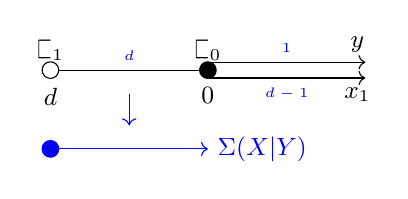
\begin{tikzpicture}[scale=1]
%edge
\draw (0,0) to (2,0);
\draw [color=blue] (1,0) node[above]{\tiny$d$};

%C_1
\draw [fill=white] (0,0) circle[radius=3pt];
\draw (0,-0.1) node[below]{\small$d$};
\draw (0,0) node[above]{\small$\sqC_1$};

%C_0
\draw [fill=black] (2,0) circle[radius=3pt];
\draw (2,-0.1) node[below]{\small$0$};
\draw (2,0) node[above]{\small$\sqC_0$};

%x_1
\draw [->] (2,0.1) -- (4,0.1);
\draw (3.9,0.1) node[above]{\small$y$};
\draw [color=blue](3,0.1) node[above]{\tiny$1$};

%y
\draw [->] (2,-0.1) -- (4,-0.1);
\draw (3.9,-0.1) node[below]{\small$x_1$};
\draw [color=blue] (3,-0.1) node[below]{\tiny$d-1$};

%down arrow
\draw [color=blue,->] (1,-0.3) -- (1,-0.7);

%target
\draw [color=blue,->] (0,-1) to (2,-1);
\draw [fill=blue,color=blue] (0,-1) circle[radius=3pt];
\draw [color=blue] (2,-1) node[right]{\small$\Sigma(X|Y)$};
\end{tikzpicture}
\end{center}
The contribution of this locus to the left-hand side of \eqref{step 2 recursion 2} is:
\begin{equation*} (d-1)\cdot(-\gamma/d) \cap [\VZ_{1,(d,\underbrace{0,\ldots,0}_{n-1})}(X|Y,\beta)].\end{equation*}
What remains on the left-hand side is a forgetful relative invariant of degree $d$ and $\leq n+1$ true markings ($y$ being the ``forgetful'' marking), hence is recursively known. On the right-hand side, the type $A$ loci are recursively known except possibly in the following special cases (with some stable distribution of the remaining non-relative markings):
\begin{center}
\begin{minipage}{0.4\textwidth}
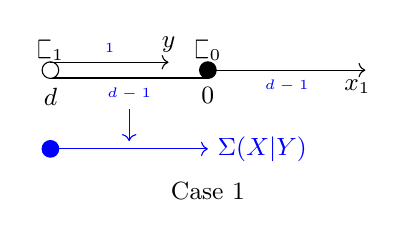
\begin{tikzpicture}[scale=1]
%edge
\draw (0,-0.1) to (2,-0.1);
\draw [color=blue] (1,-0.1) node[below]{\tiny$d-1$};

%C_1
\draw [fill=white] (0,0) circle[radius=3pt];
\draw (0,-0.1) node[below]{\small$d$};
\draw (0,0) node[above]{\small$\sqC_1$};

%C_0
\draw [fill=black] (2,0) circle[radius=3pt];
\draw (2,-0.1) node[below]{\small$0$};
\draw (2,0) node[above]{\small$\sqC_0$};

%x_1
\draw [->] (0,0.1) -- (1.5,0.1);
\draw (1.5,0.1) node[above]{\small$y$};
\draw [color=blue](0.75,0.1) node[above]{\tiny$1$};

%y
\draw [->] (2,0) -- (4,0);
\draw (3.9,0) node[below]{\small$x_1$};
\draw [color=blue] (3,0) node[below]{\tiny$d-1$};

%down arrow
\draw [color=blue,->] (1,-0.5) -- (1,-0.9);

%target
\draw [color=blue,->] (0,-1) to (2,-1);
\draw [fill=blue,color=blue] (0,-1) circle[radius=3pt];
\draw [color=blue] (2,-1) node[right]{\small$\Sigma(X|Y)$};

\draw (2,-1.3) node[below]{\small{Case 1}};
\end{tikzpicture}
\end{minipage}
\begin{minipage}{0.4\textwidth}
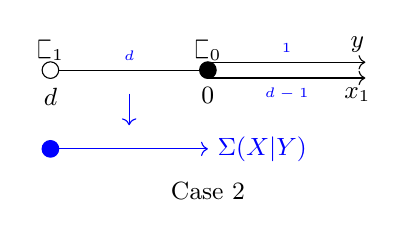
\begin{tikzpicture}[scale=1]
%edge
\draw (0,0) to (2,0);
\draw [color=blue] (1,0) node[above]{\tiny$d$};

%C_1
\draw [fill=white] (0,0) circle[radius=3pt];
\draw (0,-0.1) node[below]{\small$d$};
\draw (0,0) node[above]{\small$\sqC_1$};

%C_0
\draw [fill=black] (2,0) circle[radius=3pt];
\draw (2,-0.1) node[below]{\small$0$};
\draw (2,0) node[above]{\small$\sqC_0$};

%x_1
\draw [->] (2,0.1) -- (4,0.1);
\draw (3.9,0.1) node[above]{\small$y$};
\draw [color=blue](3,0.1) node[above]{\tiny$1$};

%y
\draw [->] (2,-0.1) -- (4,-0.1);
\draw (3.9,-0.1) node[below]{\small$x_1$};
\draw [color=blue] (3,-0.1) node[below]{\tiny$d-1$};

%down arrow
\draw [color=blue,->] (1,-0.3) -- (1,-0.7);

%target
\draw [color=blue,->] (0,-1) to (2,-1);
\draw [fill=blue,color=blue] (0,-1) circle[radius=3pt];
\draw [color=blue] (2,-1) node[right]{\small$\Sigma(X|Y)$};

\draw (2,-1.3) node[below]{\small{Case 2}};
\end{tikzpicture}
\end{minipage}
\end{center}
In Case 1 the contribution from $C_1$ is a forgetful relative invariant with $\leq n$ true markings, hence is recursively known. In Case 2, we first note that there cannot be any more markings on $C_0$ (since otherwise we could apply $\fgt_y$ and conclude that the contribution vanishes). Thus we obtain a single locus, which contributes precisely
\begin{equation*} d\cdot(-\gamma/d) \cap [\VZ_{1,(d,\underbrace{0,\ldots,0}_{n-1})}(X|Y,\beta)] = -\gamma\cap[\VZ_{1,(d,\underbrace{0,\ldots,0}_{n-1})}(X|Y,\beta)]\end{equation*}
which gives us the first term on the right-hand side of \eqref{step 2 recursion 2}. As usual the type $B$ and $C^0$ contributions are known recursively, and the only type $C^+$ contribution not known recursively occurs when the entire curve is mapped into the divisor, in which case we apply $\fgt_y$ to calculate the contribution as:
\begin{equation*} (-\gamma/d) \cap [\VZ_{1,n}(Y,\beta)] = -I/d.\end{equation*}
Substituting into \eqref{step 2 recursion 2} we end up with
\begin{equation*} I(1-d^{-1}) = \text{recursively known terms} \end{equation*}
which completes the recursion step as long as $d \neq 1$. But since $\VZ_{1,n}(H,1)=\emptyset$ it follows that $\VZ_{1,n}(Y,\beta)=\emptyset$ if $d=Y\cdot\beta=1$, so we may always assume $d \geq 2$ in the recursion.

\subsection*{Step 3} Now suppose we are given a relative space $\VZ_{1,\alpha}(X|Y,\beta)$ with an insertion $\gamma$, and suppose inductively that we have computed all forgetful relative invariants with $(d^\prime,n^\prime) \leq (d,n+1)$, all absolute invariants with $(d^\prime,n^\prime) \leq (d,n)$, all relative invariants with $(d^\prime,n^\prime,t^\prime)<(d,n,t)$ and all rubber invariants with $d^\prime < d$. Choose a true marking $x_1$ with $\alpha_1 \geq 1$ and consider the moduli space
\begin{equation*} \VZ_{1,(\alpha-e_1)\cup(1)}(X|Y,\beta) \end{equation*}
where $y$ is the newly-introduced marking. As usual consider the insertion $\tilde\gamma$ obtained from $\gamma$ by introducing $\fgt_y$ everywhere. Recursing at $x_1$ we obtain:
\begin{equation*} \left( (\alpha_1-1)\psi_1 + \ev_1^\st H\right) \tilde\gamma \cap [\VZ_{1,(\alpha-e_1)\cup(1)}(X|Y,\beta)] = \tilde\gamma \cap [\Dcal(1)].\end{equation*}
The left-hand side is a relative invariant with the same degree and number of true markings, but smaller true tangency: hence it is recursively known. On the right-hand side, the type $A$ contributions are recursively known except for those of the following form

\begin{center}
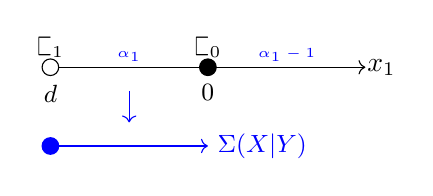
\begin{tikzpicture}[scale=1]
\draw (0,0) to (2,0);
\draw [color=blue] (1,-0.05) node[above]{\tiny$\alpha_1$};
\draw [fill=white] (0,0) circle[radius=3pt];
\draw (0,-0.1) node[below]{\small$d$};
\draw (0,0) node[above]{\small$\sqC_1$};
\draw [fill=black] (2,0) circle[radius=3pt];
\draw (2,-0.1) node[below]{\small$0$};
\draw (2,0) node[above]{\small$\sqC_0$};
\draw [->] (2,0) -- (4,0);
\draw (3.9,0) node[right]{$x_1$};
\draw [color=blue] (3,-0.05) node[above]{\tiny$\alpha_1-1$};

\draw [color=blue,->] (1,-0.3) -- (1,-0.7);

\draw [color=blue,->] (0,-1) to (2,-1);
\draw [fill=blue,color=blue] (0,-1) circle[radius=3pt];
\draw [color=blue] (2,-1) node[right]{\small$\Sigma(X|Y)$};
\end{tikzpicture}
\end{center}
where $C_0$ contains a single fictitious marking (if it had multiple fictitious markings then the contribution would vanish by projection formula) and all the other markings are on $C_1$. Thus for each fictitious marking we get a contribution of $\alpha_1 I$ where $I$ is the invariant we are trying to compute. Note that $\alpha_1 \neq 0$, and that this term appears at least once since $y$ is a fictitious marking; so we get a nonzero multiple of $I$.

As usual the type $B$ and $C^0$ contributions are recursively known. The type $C^+$ contributions are determined by lower-degree rubber invariants, except for when the whole curve is mapped into $Y$; however in this case we may apply $\fgt_y$ to identify the contribution with an absolute invariant of $Y$ with degree $d$ and $n$ markings, which is also recursively known. Thus we have determined the invariant $I$.

\subsection*{Step 4} Finally, consider a rubber space $\VZ^{\leftrightarrow}_{1,\alpha}(\mathbb P|Y_0+Y_\infty,\beta)$ with insertion $\gamma$. Suppose inductively that we have computed all absolute and relative invariants with $d^\prime \leq d$ and all rubber invariants with $(d^\prime,n^\prime,m^\prime) < (d,n,m)$.

We first note the following important reduction: if there exists a relative marking $x_k$ such that all insertions are pulled back along $\fgt_{k}$, then we may apply the projection formula, together with the fact that
\begin{equation*} (\fgt_{k})_\st [\VZ^{\leftrightarrow}_{1,\alpha}(\mathbb P|Y_0+Y_\infty,\beta)] = \alpha_k^2 \cdot [\VZ_{1,n+m-1}(Y,\beta)] \end{equation*}
to identify the rubber invariant with a multiple of a reduced invariant of $Y$, which has the same degree and hence is known recursively.

We will deal with the general case by reducing to the one above. Consider the moduli space
\begin{equation*}\label{step 4 recursion space} \VZ^{\leftrightarrow}_{1,\alpha\cup (0)}(\mathbb P|Y_0+Y_\infty,\beta)\end{equation*}
obtained by introducing a marked point $y$ with no tangency. Let $x_1$ be a positive-tangency marking (such a marking always exists since $d \geq 2$) and let $\tilde\gamma$ be the insertion obtained from $\gamma$ by replacing $\ev_1$ and $\psi_1$ by $\ev_y$ and $\psi_y$, and then introducing $\fgt_{1}^\st$ everywhere.

We will make use of a recursion formula for rubber spaces analogous to the recursion formula for relative spaces used in Steps 1--3. Following \cite{EKatz}, there is a line bundle $L_y^{\not\in \operatorname{bot}}$ on $\VZ^{\leftrightarrow}_{1,\alpha\cup (0)}(\mathbb P|Y_0+Y_\infty,\beta)$, together with a section $s_y^{\not\in\operatorname{bot}}$ whose vanishing locus consists of the locus $\Dcal(y)$ of rubber maps where $y$ is not mapped into the bottom level of the expanded target. As in \S \ref{Section Gathmann line bundle}, we can give a logarithmic interpretation of this: it corresponds to the piecewise-linear function on the tropical moduli space which associates, to every rubber tropical map, the distance between $\varphi(\sqC_y)$ and the leftmost vertex of the tropical target, where $\sqC_y$ is the vertex of the source curve containing the flag corresponding to $y$. Using this tropical description, we may easily calculate the vanshing orders of $s_y^{\not\in\operatorname{bot}}$ along the various components of $\Dcal(y)$, and show that $\cchern_1(L_y^{\not\in\operatorname{bot}}) = \Psi_0 - \ev_y^\st Y$ (see also \cite{EKatzLB}, where similar results in the non-reduced setting are obtained, using different methods). From this, we obtain a rubber recursion formula
\begin{equation}\label{step 4 recursion} (\Psi_0 - \ev_y^\st Y) \tilde\gamma \cap [\VZ^{\leftrightarrow}_{1,\alpha\cup(0)}(\mathbb P|Y_0+Y_\infty,\beta)] = \tilde\gamma \cap [\Dcal(y)]\end{equation}
where the fundamental class $[\Dcal(y)]$ is weighted by vanishing orders on the components. We will first show that the left-hand side is recursively known. By construction the class $\tilde\gamma$ is pulled back via $\fgt_{1}^\st$, and the same is true for $\ev_y^\st Y$. It remains to examine $\Psi_0$. If there exists a negative-tangency marking $x_2$, then we have \cite[Construction 5.1.17]{GathmannThesis}
\begin{equation*}\label{Psi0 formula} \Psi_0 = -\alpha_2 \hat\psi_2 - \ev_2^\st Y \end{equation*}
where $\hat\psi_2$ is a \emph{non-collapsed} psi class. (If there are no negative-tangency markings, then the construction given in \cite[\S 1.5.2]{MaulikPandharipande} shows that $\Psi_0=0$.) Now, $\hat\psi_2 - \psi_2$ is given by the loci where $x_2$ belongs to a trivial bubble. This entails a splitting of the curve into pieces, each of which contributes a rubber integral. Typically each of these pieces will have $(g^\prime,d^\prime,n^\prime,m^\prime) < (1,d,n,m)$ and hence be recursively known. The one exception is when all of the genus and degree is concentrated on the top level of the expansion, with the bottom level containing only a single non-relative marking in addition to all the negative-tangency markings. But in this case the contribution is a rubber invariant where all of the insertions are pulled back via $\fgt_1^\st$, and hence we may apply the projection formula to identify this with an absolute invariant of $Y$ which is recursively known. We conclude that, up to recursively knwon terms, we may replace $\hat\psi_2$ by $\psi_2$ in the left-hand side of \eqref{step 4 recursion}. If we now compare $\psi_2$ with $\fgt_1^\st \psi_2$ we see that the difference is given by the locus where $x_1$ and $x_2$ belong to a collapsed rational piece. The contribution of this locus consists of rubber invariant with strictly fewer relative markings, and hence is recursively known. So up to recursively-known terms \eqref{step 4 recursion} becomes
\begin{equation*} \fgt_1^\st (-\alpha_2\psi_2 - \ev_y^\st Y)\tilde\gamma \cap [\VZ^{\leftrightarrow}_{1,\alpha\cup(0)}(\mathbb P|Y_0+Y_\infty,\beta)] = \tilde\gamma\cap[\Dcal(y)]\end{equation*}
and now the left-hand side is also recursively known, by the projection formula. Let us now examine the right-hand side. The components of $\Dcal(y)$ are indexed by splittings of the curve, and certainly the contributions are recursively known unless there is a piece of the curve carrying all of the genus and degree, so we may restrict to examining these contributions.

Let us denote the piece of the curve carrying all of the genus and degree by $C^\prime\subseteq C$. If $C^\prime$ is mapped to top level, then either it contains $x_1$, in which case we apply $\fgt_1$ to compute the contribution, or it does not contains $x_1$, in which case it has fewer than $n$ relative markings and is known recursively.  If on the other hand $C^\prime$ is not mapped to top level, then generically it is mapped to the bottom level (since generically the core is not contracted on this locus, so the desingularisation process does nothing). One possible contribution is given by the following locus
\begin{center}
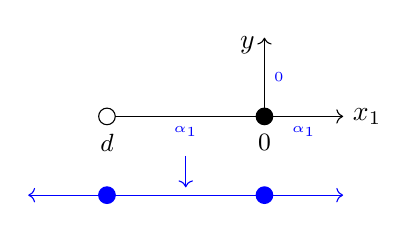
\begin{tikzpicture}[scale=1]
%edge
\draw (0,0) to (2,0);
\draw [color=blue] (1,0) node[below]{\tiny$\alpha_1$};

%C_1
\draw [fill=white] (0,0) circle[radius=3pt];
\draw (0,-0.1) node[below]{\small$d$};

%y
\draw [->] (2,0) -- (2,1);
\draw (2,0.9) node[left]{$y$};
\draw [color=blue] (2,0.5) node[right]{\tiny$0$};

%x_1
\draw [->] (2,0) -- (3,0);
\draw (3,0) node[right]{$x_1$};
\draw [color=blue] (2.5,0) node[below]{\tiny$\alpha_1$};

%C_0
\draw [fill=black] (2,0) circle[radius=3pt];
\draw (2,-0.1) node[below]{\small$0$};

%down arrow
\draw [color=blue,->] (1,-0.5) -- (1,-0.9);

%target
\draw [color=blue] (0,-1) to (2,-1);
\draw [fill=blue,color=blue] (0,-1) circle[radius=3pt];
\draw [fill=blue,color=blue] (2,-1) circle[radius=3pt];
\draw [color=blue,->] (2,-1) -- (3,-1);
\draw [color=blue,->] (0,-1) -- (-1,-1);
\end{tikzpicture}
\end{center}
which contributes a nonzero multiple of the invariant $I$ we are trying to compute. For the other possibilities, first note that, unless every component at the top level contains a single positive-tangency marking and a single node (together with possibly some tangency-zero markings), then $C^\prime$ has fewer than $n$ relative markings and hence the contribution is known recursively. On the other hand, if any non-relative marking other than $y$ is mapped to the top level, $C^\prime$ has $\leq n$ relative markings and less than $m$ non-relative markings, and hence again the contribution is known recursively. The only remaining possibilities are when $x_1$ is replaced by another positive-tangency marking $x_k$ in the above picture; but then the contribution can be calculated by applying the projection formula to $\fgt_{1}$. We therefore conclude that the only contribution to the right-hand side of \eqref{step 4 recursion} which is not known recursively is a nonzero multiple of the invariant we were trying to compute. This completes the recursion step.

\bibliographystyle{alpha}
\bibliography{Bibliography}

\bigskip\bigskip

\noindent Luca Battistella\\
Max-Planck-Institut f\"ur Mathematik, Bonn \\
\href{mailto:battistella@mpim-bonn.mpg.de}{battistella@mpim-bonn.mpg.de}\\

\noindent Navid Nabijou \\
School of Mathematics and Statistics, University of Glasgow \\
\href{mailto:Navid.Nabijou@glasgow.ac.uk}{navid.nabijou@glasgow.ac.uk}\\

\noindent Dhruv Ranganathan \\
Department of Pure Mathematics and Mathematical Statistics, University of Cambridge \\
\href{mailto:dr508@cam.ac.uk}{dr508@cam.ac.uk}

\end{document}